% Wczytanie szablonu
\documentclass[nostrict,polish]{Szablon}

% Definicja dokumentu
\usepackage[unicode=true]{hyperref}
\newcommand\PDFtitle{Silnik renderujący używający technik cieniowania odroczonego}
\newcommand\PDFauthors{Szymon Szczyrbak}
\hypersetup{
  pdftitle={\PDFtitle},
  pdfauthor={\PDFauthors},
}

% Biblatex
\usepackage{babel}
\usepackage{biblatex}

% Diagramy
\usepackage{tikz}
\usepackage{float}
\usetikzlibrary{er,positioning,fit,shapes.multipart,calc,decorations.text}

% Usuń list spacing
\raggedbottom

% StrSubstitute
\usepackage{xstring}
\newcommand\myesc[1]{\StrSubstitute{#1}{_}{\textunderscore}}

% Napraw marginesy
\renewcommand\_{\textunderscore\allowbreak}

% includepdf
\usepackage{pdfpages}

% |c|>{\Raggedright}p{1cm}|c}
\usepackage{array}
\usepackage[originalparameters]{ragged2e}

% listingi

\usepackage{listings}

% Napraw polskie znaki w listingach: https://tex.stackexchange.com/questions/652497/troubles-with-listings-and-polish-characters-lualatex
\makeatletter
\lst@InputCatcodes
\def\lst@DefEC{%
	\lst@CCECUse \lst@ProcessLetter
	^^80^^81^^82^^83^^84^^85^^86^^87^^88^^89^^8a^^8b^^8c^^8d^^8e^^8f%
	^^90^^91^^92^^93^^94^^95^^96^^97^^98^^99^^9a^^9b^^9c^^9d^^9e^^9f%
	^^a0^^a1^^a2^^a3^^a4^^a5^^a6^^a7^^a8^^a9^^aa^^ab^^ac^^ad^^ae^^af%
	^^b0^^b1^^b2^^b3^^b4^^b5^^b6^^b7^^b8^^b9^^ba^^bb^^bc^^bd^^be^^bf%
	^^c0^^c1^^c2^^c3^^c4^^c5^^c6^^c7^^c8^^c9^^ca^^cb^^cc^^cd^^ce^^cf%
	^^d0^^d1^^d2^^d3^^d4^^d5^^d6^^d7^^d8^^d9^^da^^db^^dc^^dd^^de^^df%
	^^e0^^e1^^e2^^e3^^e4^^e5^^e6^^e7^^e8^^e9^^ea^^eb^^ec^^ed^^ee^^ef%
	^^f0^^f1^^f2^^f3^^f4^^f5^^f6^^f7^^f8^^f9^^fa^^fb^^fc^^fd^^fe^^ff%
	żłćęśąźń%
	^^00}
\lst@RestoreCatcodes
\makeatother

%% Copyright (c) 2020-2021 Benno Bielmeier
%% SPDX-License-Identifier: MIT
%%
%% GLSL definition
%%
\lstdefinelanguage{GLSL}%
{%
	morekeywords={%
		% Layouts
		layout, std140, std430, scalar, set, binding, uniform,
		% HLSL constants
		false,FALSE,NULL,true,TRUE,%
		% GLSL predefinde macro constant
		__LINE__,__FILE__,__VERSION__,GL_core_profile,GL_es_profile,GL_compatibility_profile,%
		% GLSL precision modifier
		precision,highp,mediump,lowp,%
		% GLSL control keywords
		break,case,continue,default,discard,do,else,for,if,return,switch,while,%
		% GLSL types
		void,bool,int,uint,float,double,vec2,vec3,vec4,dvec2,dvec3,dvec4,bvec2,bvec3,bvec4,ivec2,ivec3,ivec4,uvec2,uvec3,uvec4,mat2,mat3,mat4,mat2x2,mat2x3,mat2x4,mat3x2,mat3x3,mat3x4,mat4x2,mat4x3,mat4x4,dmat2,dmat3,dmat4,dmat2x2,dmat2x3,dmat2x4,dmat3x2,dmat3x3,dmat3x4,dmat4x2,dmat4x3,dmat4x4,sampler1D,sampler2D,sampler3D,image1D,image2D,image3D,samplerCube,imageCube,sampler2DRect,image2DRect,sampler1DArray,sampler2DArray,image1DArray,image2DArray,samplerBuffer,imageBuffer,sampler2DMS,image2DMS,sampler2DMSArray,image2DMSArray,samplerCubeArray,imageCubeArray,sampler1DShadow,sampler2DShadow,sampler2DRectShadow,sampler1DArrayShadow,sampler2DArrayShadow,samplerCubeShadow,samplerCubeArrayShadow,isampler1D,isampler2D,isampler3D,iimage1D,iimage2D,iimage3D,isamplerCube,iimageCube,isampler2DRect,iimage2DRect,isampler1DArray,isampler2DArray,iimage1DArray,iimage2DArray,isamplerBuffer,iimageBuffer,isampler2DMS,iimage2DMS,isampler2DMSArray,iimage2DMSArray,isamplerCubeArray,iimageCubeArray,atomic_uint,usampler1D,usampler2D,usampler3D,uimage1D,uimage2D,uimage3D,usamplerCube,uimageCube,usampler2DRect,uimage2DRect,usampler1DArray,usampler2DArray,uimage1DArray,uimage2DArray,usamplerBuffer,uimageBuffer,usampler2DMS,uimage2DMS,usampler2DMSArray,uimage2DMSArray,usamplerCubeArray,uimageCubeArray,struct,%
		% GLSL support variables
		gl_BackColor,gl_BackLightModelProduct,gl_BackLightProduct,gl_BackMaterial,gl_BackSecondaryColor,gl_ClipDistance,gl_ClipPlane,gl_ClipVertex,gl_Color,gl_DepthRange,gl_DepthRangeParameters,gl_EyePlaneQ,gl_EyePlaneR,gl_EyePlaneS,gl_EyePlaneT,gl_Fog,gl_FogCoord,gl_FogFragCoord,gl_FogParameters,gl_FragColor,gl_FragCoord,gl_FragData,gl_FragDepth,gl_FrontColor,gl_FrontFacing,gl_FrontLightModelProduct,gl_FrontLightProduct,gl_FrontMaterial,gl_FrontSecondaryColor,gl_InstanceID,gl_Layer,gl_LightModel,gl_LightModelParameters,gl_LightModelProducts,gl_LightProducts,gl_LightSource,gl_LightSourceParameters,gl_MaterialParameters,gl_ModelViewMatrix,gl_ModelViewMatrixInverse,gl_ModelViewMatrixInverseTranspose,gl_ModelViewMatrixTranspose,gl_ModelViewProjectionMatrix,gl_ModelViewProjectionMatrixInverse,gl_ModelViewProjectionMatrixInverseTranspose,gl_ModelViewProjectionMatrixTranspose,gl_MultiTexCoord0,gl_MultiTexCoord1,gl_MultiTexCoord2,gl_MultiTexCoord3,gl_MultiTexCoord4,gl_MultiTexCoord5,gl_MultiTexCoord6,gl_MultiTexCoord7,gl_Normal,gl_NormalMatrix,gl_NormalScale,gl_ObjectPlaneQ,gl_ObjectPlaneR,gl_ObjectPlaneS,gl_ObjectPlaneT,gl_Point,gl_PointCoord,gl_PointParameters,gl_PointSize,gl_Position,gl_PrimitiveIDIn,gl_ProjectionMatrix,gl_ProjectionMatrixInverse,gl_ProjectionMatrixInverseTranspose,gl_ProjectionMatrixTranspose,gl_SecondaryColor,gl_TexCoord,gl_TextureEnvColor,gl_TextureMatrix,gl_TextureMatrixInverse,gl_TextureMatrixInverseTranspose,gl_TextureMatrixTranspose,gl_Vertex,gl_VertexID,%
		% GLSL support constants
		gl_MaxClipPlanes,gl_MaxCombinedTextureImageUnits,gl_MaxDrawBuffers,gl_MaxFragmentUniformComponents,gl_MaxLights,gl_MaxTextureCoords,gl_MaxTextureImageUnits,gl_MaxTextureUnits,gl_MaxVaryingFloats,gl_MaxVertexAttribs,gl_MaxVertexTextureImageUnits,gl_MaxVertexUniformComponents,%
		% GLSL support functions
		abs,acos,all,any,asin,atan,ceil,clamp,cos,cross,degrees,dFdx,dFdy,distance,dot,equal,exp,exp2,faceforward,floor,fract,ftransform,fwidth,greaterThan,greaterThanEqual,inversesqrt,length,lessThan,lessThanEqual,log,log2,matrixCompMult,max,min,mix,mod,noise1,noise2,noise3,noise4,normalize,not,notEqual,outerProduct,pow,radians,reflect,refract,shadow1D,shadow1DLod,shadow1DProj,shadow1DProjLod,shadow2D,shadow2DLod,shadow2DProj,shadow2DProjLod,sign,sin,smoothstep,sqrt,step,tan,texture1D,texture1DLod,texture1DProj,texture1DProjLod,texture2D,texture2DLod,texture2DProj,texture2DProjLod,texture3D,texture3DLod,texture3DProj,texture3DProjLod,textureCube,textureCubeLod,transpose,%
		% GLSL struct member -> FixMe: Should have dot(.) as delimiter
		rgb
	},
	sensitive=true,%
	morecomment=[s]{/*}{*/},%
	morecomment=[l]//,%
	morestring=[b]",%
	morestring=[b]',%
	moredelim=*[directive]\#,%
	% keyword.control.hlsl
	moredirectives={define,defined,elif,else,if,ifdef,endif,line,error,ifndef,include,pragma,undef,warning,extension,version}%
}[keywords,comments,strings,directives]%

\lstdefinelanguage{SPIRV}
{
	morekeywords={
		OpCapability, Shader, RuntimeDescriptorArray,
		OpExtension,
		OpName,
		OpDecorate, DescriptorSet, Binding,
		OpTypeImage, 
		OpTypeSampledImage,
		OpTypeRuntimeArray,
		OpTypePointer, UniformConstant,
		OpVariable
	},
	morestring=[b]",
	sensitive=true
}

\lstdefinelanguage{json}
{
	morestring=[b]",
	morestring=[d]'
}

\lstdefinelanguage{verbatim}
{
	basicstyle=\ttfamily,
	columns=fullflexible,
	keepspaces=true,
	inputencoding=utf8,
	extendedchars=true,
}

% Część właściwa pracy
\begin{document}

\includepdf[pages=-]{StronaTytulowaPG}
\chapter*{Streszczenie}
\addcontentsline{toc}{chapter}{Streszczenie}  

\chapter*{Abstract}
\addcontentsline{toc}{chapter}{Abstract}  

\chapter*{Spis treści}
\addcontentsline{toc}{chapter}{Spis treści}

\tableofcontents

\chapter*{Wykaz ważniejszych oznaczeń i skrótów}
\addcontentsline{toc}{chapter}{Wykaz ważniejszych oznaczeń i skrótów}

Skróty:
\begin{itemize}
\item{API} - Application Programming Interface, interfejs programistyczny aplikacji;
\item{CPU} - Central Processing Unit, procesor;
\item{CTS} - Conformance Test Suite, pakiet testów zgodności;
\item{GPU} - Graphics Processing Unit, procesor graficzny.
\item{IHV} - Independent Hardware Vendor, niezależny dostawca sprzętu,
\item{ISA} - Instruction Set Architecture, architektura procesora,
\item{GLSL} - OpenGL Shading Language, język programowania potoku graficznego wprowadzony w API OpenGL,
\item{HLSL} - High-Level Shader Language, język programowania potoku graficznego wprowadzony w API Direct3D 9,
\item{SDK} - Software Development Kit, zestaw narzędzi dla programistów aplikacji.
\end{itemize}
\chapter{Wstęp}
\label{chap:introduction}

Podręcznik \cite{HughesDamEtAl13} definiuje grafikę komputerową jako dziedzinę interdyscyplinarna zajmującą się komunikacją wizualną za pomocą wyświetlacza komputera i jego urządzeń wejścia-wyjścia.

Rozwój teoretyczny grafiki komputerowej jest zdominowany przez doroczną konferencję SIGGRAPH \cite{SIGGRAPH}, podczas której prezentacje i dyskusje akademickie są przeplecione z targami branżowymi.
Rozwój grafiki komputerowy jest w znacznej mierze napędzany wymaganiami stawianymi przez przemysł rozrywkowy. Przykładem jest dobrze znana seria kursów przeznaczona dla twórców gier komputerowych obejmująca najnowsze prace i postępy w technikach renderowania czasu rzeczywistego używanych w silnikach graficznych rozwijanych przez producentów gier komputerowych \cite{SIGGRAPH_ADVANCES}.

Renderowanie to proces konwersji pewnych prymitywów na obraz przeznaczony do wyświetlania na ekranie.
Wyświetlany obraz jest nazywany klatką (ang. frame).

Renderowanie czasu rzeczywistego nakłada ograniczenie czasowe dotyczące liczby klatek na sekundę (ang. frames per second, FPS), która musi być na tyle wysoka, by dawać iluzję ciągłości ruchu.
Przyjmuje się, że ograniczenie to jest spełniane poprzez zapewnienie wyświetlanie minimum 30 klatek na sekundę (renderowanie trwa krócej niż $\frac{1}{30}$ sekundy).
Eliminuje to kosztowne obliczeniowo techniki renderowania dające fotorealisteczne rezultaty takie jak śledzenie promieni (ang. ray tracking) i wymaga od programistów zastosowania technik aproksymacji mniej lub bardziej luźno opertych na prawach fizyki oraz użycia bibliotek graficznych wspierających eerację sprzętową takich jak Vulkan lub OpenGL.

Silnik renderujący, zwany też silnikiem graficznym to element aplikacji odpowiadający za renderowanie czasu rzeczywistego. Zapewnia on wysokopoziomową warstwę abstrakcji pozwalającą użytkownikowi na operowanie używając takich konceptów jak sceny, obiekty, materiały lub światła oraz ukrywają niskopoziomowe detale użytych bibliotek i technik graficznych.

Zaprojektowanie i zaimplementowanie silnika graficznego jest złożonym procesem wymagającym znajomości szerokiego wachlarza technik graficznych z całego możliwego spektrum poziomów abstrakcji, dlatego też coraz więcej twórców gier komputerowych decyduje się na licencjonowanie i użycie gotowego silnika graficznego zamiast powolnej i mozolnej pracy nad własnymi rozwiązaniami.

Jeśli jednak celem inżyniera jest poszerzenie osobistego zrozumienia grafiki komputerwej, to warto podjąć próbę stworzenia własnego silnika graficznego.


\section{Cel pracy}

Celem pracy jest zaprojektowanie i zaimplementowanie silnika graficznego, którego potok graficzny używa techniki cieniowania odroczonego.

Silnik został napisana jako biblioteka programistyczna języka C używającej skryptów Python do automatycznej generacji kodu podczas procesu budowania.
Renderowanie grafiki 3D jest obsługiwane przez Vulkan API.
Zasoby uzywane podczas renderowania są wczytywane z bazy zasobów, która jest wyjściem potoku zasobów działającego podczas procesu budowania.
Działanie biblioteki jest sterowane plikiem konfiguracyjnym dostarczonym przez użytkownika i jest demonstrowane przy użyciu pliku wykonywalnego renderujacego przykładową scenę używając cieniowania odroczonego.

Celem autora było zapoznanie się z teorią stojącą za elementami składającymi się na silnik graficzny i praktyczne zademonstrowanie zdobytej wiedzy.


\section{Zakres pracy}

Niniejsza praca ma charakter przeglądowy. Nowoczesne silniki graficzne składają się z wielu elementów, z których każdy może być niezależnie rozwijany do dowolnie wysokiego poziomu skomplikowania, dlatego trudno je wszystkie dokładnie i wyczerpująco opisać w ramach jednej pracy.

Zakres pracy obejmuje:
\begin{itemize}
	\item {opis algorytmów i technik graficznych używanych w nowoczesnych silnikach graficznych, ze szczególnym naciskiem na Vulkan API i renderowanie odroczone},
	\item{omówienie architektury i implementacji projektu},
	\item{demonstrację użycia silnika graficznego do wyrenderowania przykładowej sceny},
	\item{analizę wydajności silnika graficznego}.
\end{itemize}

Stworzony silnik nie może konkurować z silnikami graficznymi profesjonalnie rozwijanymi przez duże drużyny z myślą o zastosowaniu w grach komputerowych (takimi jak otwarty Godot \cite{godotengine} czy komercyjny Unreal Engine \cite{unrealengine}).
Jest on jednak przystosowany do względnie łatwej, szybkiej i elastycznej modyfikacji potoku graficznego oraz wspiera mechanizmy zgłaszania informacji debugowania oferowane przez Vulkan API, co pozwala na szybki cykl prototypowania i debugowania podczas zapoznawania się z technikami graficznymi.

\section{Struktura pracy}


Praca została podzielona na pięć rozdziałów, z których każdy jest rozwinięciem rozdziału poprzedniego.

Pierwszy rozdział pracy definiuje cel, zakres i strukturę pracy.

Drugi rozdział zawiera wprowadzenie do wybranych części dziedziny grafiki komputerowej użytych podczas późniejszej implementacji silnika renderującego.

W trzecim rozdziale opisano architekturę silnika i szczegóły implementacji poszczególnych jego modułów.

W trzecim rozdziale opisano specyficzny potok graficzny używający cieniowania odroczonego do realizacji modelu oświetlenia
opartego o renderowanie bazujące na fizyce.

W czwartym rozdziale wyrenderowano przykładową scenę i zbadano wydajność
silnika.

Ostatni rozdział zawiera podsumowanie oraz opis przewidywanych kierunków przyszłego rozwoju silnika.





\chapter{Wprowadzenie do dziedziny}
\label{chap:field}

Grafika komputerowa czasu rzeczywistego jest szerokim zagadnieniem.
W tym rozdziale przybliżono podstawowe pojęcia, bibliotekę Vulkan oraz techniki renderowania, których zrozumienie jest wymagane przed rozpoczęciem implementacji silnika graficznego.

\section{Podstawowe pojęcia}
// TODO matematyka
// TODO podział przestrzeni

\section{Vulkan}

Biblioteki graficzne pozwalaja aplikacji na użycie ich API do uzyskania dostępu do akceleracji sprzętowej, czyli przeniesienia obliczeń wymaganych przez renderowanie z CPU do specjalnie pod nie zoptymalizowanego GPU.

Biblioteka graficzna mająca na celu równe wsparcie wielu platform rozwijanych przez różnych IHV (\textit{Independent Hardware Vendor}, niezależny dostawca sprzętu) wymaga drobiazgowego ustandaryzowania i dokumentacji.
W czasie pisania pracy istnieją trzy popularne standardy: Direct3D od firmy Microsoft oraz OpenGL i Vulkan od konsorcjum non-profit Khronos.

Vulkan w wersji 1.0 został po raz pierwszy wydany w 2016. By zacząć używać Vulkan należy pobrać Vulkan SDK rozwijany przez LunarG \cite{VULKANSDK}.
Zawiera on m.in. specyfikację, nagłówki API, biblioteki (de)kompilujące kod SPIR-V oraz warstwy walidacji.

\paragraph{Specyfikacja}

Specyfikacja Vulkan \cite{VULKANSPEC} to ponad 1000 stron zwięzłej, precyzyjnej i szczgółowej specyfikacji API przeznaczonej do użytku zarówno przez implementatorów sterowników, jak i programistów aplikacji. Khronos utrzymuje listę urządzeń, które zaliczyły zestaw testów zgodności Vulkan CTS \cite{VULKANCTS} i spełniają wymagania wieloplatformowości (w odróżnieniu takich API jak DirectX wspieranego tylko przez system Windows i konsole Xbox \cite{HughesDamEtAl13} czy Metal wspierane przeez urządzenia firmy Apple).

\paragraph{Obiektowość i bezstanowość}

Vulkan jest API obiektowym - wszystkie używane koncepty są reprezentowane przez obiekty Vulkan tworzone i niszczone przez aplikację, która ma do nich dostęp poprzez uchwyty.
W przeciwieństwie do OpenGL używającego globalnej maszyny stanów,

Vulkan jest bezstanowy, używany stan jest całkowiecie zaszyty w obiektach i wszystkie funkcje API operują tylko stanie obiektów przekazanych do nich w postaci parametrów i mogą być wywoływane współbieżnie z wielu wątków. Wyjątkiem są parametry zdefiniowane jako \textit{zewnętrznie synchronizowane}, dla których aplikacja musi zagwarantować, że tylko jeden wątek używa obiektu takiego parametu w danym momencie - przykładowo większość funkcji nagrywania poleceń \textit{vkCmd*} wymagają zewnętrznej synchronizacji obiektu bufora poleceń \textit{VkCommandBuffer}, co oznacza, że nagrywanie pojedyńczego bufora poleceń powinno się najlepiej odbywać w ramach jednego wątku.

\paragraph{SPIR-V}

Vulkan używa niskopoziomowej pośredniej reprezentacji shaderów w postaci kodu bajtowego SPIR-V \cite{SPIRVSPEC}, który jest standardem Khronos będącym przenośnym celem kompilacji shaderów napisanych w wysokopoziomowych językach takich jak GLSL, HLSL czy Cg.
Implementatorzy zajmują się tylko translację ze SPIR-V do kodu maszynowego urządzenia, co znacznie upraszcza sterowniki niemuszące osadzać całego kompilatora, przyśpiesza proces kompilacji oraz zmniejsza prawdopodobieństwo sytuacji znanej z OpenGL, w której mimo deklarowanej przenośności API sterowniki różnej jakości interpretują ten sam shader na różne sposoby \cite{GLSLBAD}.

\paragraph{Warstwy}

Vulkan jest niskopioziomowy i skomplikowany w użyciu - słynny tutorial wymaga ponad 1000 linijek kodu C++ do renderowania pojedyńczego trójkąta  \cite{VULKANTUTORIAL}.
Sterowniki nie sprawdzają większości błędów i wymagają od programisty chcącego uniknąć korupcji drobiazgowego przestrzegania zasad poprawnego użycia API.

Na szczęście Vulkan wspiera tworzenie warstw - małych bibliotek dynamicznych pośredniczących pomiędzy apikacją i sterownikiem, które przechwytują wywołania API i pozwala na dodanie do nich dodatkowej logiki.
Vulkan SDK oferuje oficjalne warstwy mające uprościć proces debugowania.

Warstwa walidacji \textit{VK\_LAYER\_KHRONOS\_validation} wykrywaja i raportuje nieprawidłowe i niewydajne użycie API.

Warstwy rozszerzeń implementują funkcje rozszerzeń niewspieranych przez sterownik - przykładowo warstwa \textit{VK\_LAYER\_KHRONOS\_synchronization2} implementuje rozszerzenie \textit{VK\_KHR\_synchronization2}.

Warstwy narzędzi dodają przydatne funkcjonalności takie jak raportowanie wywołań API (\textit{VK\_LAYER\_LUNARG\_api\_dump}), robienie zrzutów ekranu (\textit{VK\_LAYER\_LUNARG\_screenshot}) czy symulacja możliwości bardziej ograniczonych GPU (\textit{VK\_LAYER\_LUNARG\_device\_simulation}).

Warstwy mają negatywny wpływ na wydajność, który jest zwłaszcza widoczny w przypadku warstwy walidacji. Dlatego też warto używać je w trakcie rozwoju, ale nie w produkcie końcowym.

\paragraph{Rozszerzenia}

Nowa funkcjonalność jest dodawana podobnie jak w OpenGL uzywając opcjonalnych rozszerzeń podstawowej specyfikacji. Są one proponowane przez członków Khronos i często są specyficzne dla urządzeń - przykładowo rozszerzenie \textit{VK\_NV\_mesh\_shader} pozwala na użycie shaderów siatki na GPU firmy Nvidia.

Rozszerzenia \textit{EXT} są wspierane przez wielu dostawców. Dostatecznie popularne rozszerzenie może stać się podstawą rozszerzenia \textit{KHR}, od którego oczekuje się wsparcia przez większość sterowników - przykładowo na podstawie rozszerzenia \textit{VK\_NV\_ray\_tracing} stworzono rozszerzenie \textit{VK\_KHR\_ray\_tracing\_pipeline}.

Rozszerzenia mogą być promowana w nowej wersji Vulkan stając się częścią postawowej specyfikacji - przykładowo rozszerzenie \textit{VK\_EXT\_scalar\_block\_layout} zostało promowane w Vulkan 1.2.

\subsection{Podstawy API}

API Vulkan posiadaja regularną i przewidywalną strukturę nazewnictwa oraz użycia obieków.

\subsubsection{Konwencje nazewnictwa}
Konwencje nazewnictwa API Vulkan posiadają regularną i przewidywalną strukturę.
Nagłówek \textit{vulkan.h} dołącza funkcje, struktury, typy wyliczeniowe i stałe preprocesora języka C mające następujące przedrostki:
\begin{itemize}
	\item \textit{vk}: funkcje (np. \textit{vkBeginCommandBuffer}),
	\item \textit{Vk}: struktury i typy wyliczeniowe (np. \textit{VkPipeline} i  \textit{VkPipelineBindPoint}),
	\item \textit{VK\_}: wyliczenia i stałe (np. \textit{VK\_PIPELINE\_BIND\_POINT\_GRAPHICS} i \textit{VK\_NULL\_HANDLE}),
\end{itemize}
W imię zwięzłości dalej w pracy części nazwy będą pomijane jeśli można je wywnioskować z kontekstu - przykładowo \textit{VK\_PIPELINE\_STAGE\_COLOR\_ATTACHMENT\_OUTPUT\_BIT} może być zapisywany jako etap potoku \textit{COLOR\_ATTACHMENT\_OUTPUT}.

Funkcje \textit{vkCmd*()} są nazywane poleceniami i nagrywają polecenie przeznaczone do wykonania na GPU do bufora poleceń - przykładowo polecenie \textit{vkCmdCopyBufferToImage} nagrywa polecenie kopiowania bufora do obrazu.

Funkcje \textit{vkEnumerate*()} i \textit{vkGet*()} służą do odpytywania właściwości obiektów - przykładowo funkcja \textit{vkGetPhysicalDeviceQueueFamilyProperties()} raportuje właściwości rodzin kolejek udostępnianych przez dane urządzenie fizyczne.

Nowe elementy nagłówka wprowadzane przez rozszerzenia kończą się przyrostkami - przykładowo rozszerzenie \textit{VK\_NV\_device\_diagnostic\_checkpoints} wprowadza funkcję \textit{vkCmdSetCheckpointNV} używającą struktury \textit{VkCheckpointDataNV}.

\subsubsection{Model obiektów}

Wszystkie obiekty Vulkan mogą być albo tworzone funkcją \textit{vkCreate*()}, albo alokowane z puli wcześniej utworzonego obiektu funkcją \textit{vkAllocate*()}.

Tworzenie obiektu wymaga przygotowania struktury informacji tworzenia \textit{Vk*CreateInfo}:
\lstset{language=C}
\begin{lstlisting}
Vk*CreateInfo createInfo = {
	.sType = VK_STRUCTURE_TYPE_*_CREATE_INFO;
	.flags = ...,
	...
	.pNext = NULL,
};

Vk* object;
assert(vkCreate*(..., &createInfo, ..., &object) == VK_SUCCESS);
\end{lstlisting}

Alokacja obiektu wymaga przygotowania struktury informacji alokacji \textit{Vk*AllocateInfo}:
\lstset{language=C}
\begin{lstlisting}
Vk*Pool pool;

Vk*AllocateInfo allocInfo = {
	.sType = VK_STRUCTURE_TYPE_*_ALLOCATE_INFO;
	.*Pool = pool,
	...
	.pNext = NULL,
};

Vk* object;
assert(vkAllocate*(..., &allocInfo, ..., &object) == VK_SUCCESS);
\end{lstlisting}

Stworzone obiekty są niszczone funkcją \textit{vkDestroy*()}.
Zaalokowane obiekty są zwalniane funkcją \textit{vkFree*()} lub poprzez zniszczenie puli obiektów.

Struktury Vulkan często wspierają łańcuch \textit{pNext} - wskaźnik \textit{void*} na kolejną strukturę w liście jednokierunkowej lub \textit{NULL}. Jest on używany przez rozszerzenia dodające nowe struktury i może być iterowany w wygodny sposób używając struktur \textit{VkBaseInStructure} i \textit{VkBaseOutStructure} - typ stuktury może być wywnioskowany używając jej pierwszego pola \textit{sType}.

\subsection{Szkielet aplikacji graficznej}

Vulkan, z racji swojej niskopoziomowości, nie narzuca jednej konkretnej struktury aplikacji - większość problemów można rozwiązać wieloma technikami, z których każda ma swoje zalety i wady.
Programista powinien zaprojektować program w taki sposób, żeby rozwiązywał on problem, nie był zawiły i jego profilowanie ujawniało maksymalne użycie GPU.

Wszystkie aplikacjie graficzne mogą być jednak podsumowane następującymi ogólnymi krokami:
\begin{itemize}
	\item Stworzenie bądź wybór podstawowych obiektów: instancja (\textit{VkInstance}), urządzenie fizyczne (\textit{VkPhysicalDevice}), urządzenie logiczne (\textit{VkDevice}) oraz kolejka graficzna (\textit{VkQueue}),
	\item Przygotowanie obiektów służących do prezentacji wyników renderowania: powierzchnia okna (\textit{VkSurface}), łańcuch wymiany (\textit{VkSwapchain}), prezentowalne obrazy (\textit{VkImage}) i ich widoki (\textit{VkImageView}) oraz kolejka prezentacji (\textit{VkQueue}),
	\item Transfer zasobów z CPU do GPU opisanych w zbiorach deskryptorów (\textit{VkDescriptorSet}),
	\item Stworzenie obiektów opisujących proces renderowania: potoki (\textit{VkPipeline}) z shaderami (\textit{VkShaderModule}) oraz przebiegi renderowania (\textit{VkRenderPass}),
	\item Wykonanie procesu renderowania w pętli głównej programu: pobranie nieużywanego prezentowalnego obrazu, nagranie i wykonanie buforów poleceń (\textit{VkCommandBuffer}) realizujących pożądane techniki renderowania oraz prezentacja wyrenderowaniego obrazu.
\end{itemize}

W kolejnych sekcjach pracy przybliżono wspomniane powyżej obiekty Vulkan i zaprezentowano metody ich użycia.


\subsection{Inicjalizacja podstawowych obiektów}

Wszyskie programy używające API Vulkan wymagają wcześniejszego stworzenia obiektów w następującej kolejności:
\begin{itemize}
	\item instancji (\textit{VkInstance}),
	\item powierzchni okna (\textit{VkSurface}),
	\item urządzenia fizycznego (\textit{VkPhysicalDevice}),
	\item urządzenia logicznego (\textit{VkDevice}),
	\item wskaźników funkcji rozszerzeń,
	\item kolejek (VkQueue),
\end{itemize}

Poniższy diagram przedstawia kolejność inicjalizacji podstawowych obiektów Vulkan:
\begin{figure}[H]
	\centering
	\begin{tikzpicture}[node distance=1cm]
		\tikzstyle{object} = [rectangle, minimum width=3cm, minimum height=1cm,text centered, draw=black]
		\tikzstyle{input} = [rectangle, rounded corners, minimum width=3cm, minimum height=5mm,text centered, draw=black]
		\tikzstyle{arrow} = [thick,->,>=stealth]
		\tikzstyle{relation} = [densely dotted,->]
		
		\node (VkInstance) [object] {VkInstance};
		\node (VkApplicationInfo) [input, above = 3mm of VkInstance, rectangle split, rectangle split parts=3] {VkApplicationInfo\nodepart{two}Rozszerzenia instancji\nodepart{three}Warstwy};
		\node (VkSurface) [object, right = of VkInstance] {VkSurface};
		\node (WSI) [input, above = 3mm of VkSurface] {Rozszerzenia WSI};
		\node (VkPhysicalDevice) [object, below = of VkInstance] {VkPhysicalDevice};
		\node (VkDevice) [object, right = of VkPhysicalDevice] {VkDevice};
		\node (VkDeviceInfo) [input, below = 3mm of VkDevice, rectangle split, rectangle split parts=4] {Rodziny kolejek\nodepart{two}Funkcjonalności\nodepart{three}Rozszerzenia urządzenia\nodepart{four}Warstwy};
		\node (VkQueue) [object, right = of VkDevice] {VkQueue};
		
		\draw [arrow] (VkApplicationInfo) -- (VkInstance);
		\draw [arrow] (VkInstance) -- (VkSurface);
		\draw [arrow] (WSI) -- (VkSurface);
		\draw [relation] (VkInstance) -- (VkPhysicalDevice);
		\draw [relation] (VkSurface) -- (VkPhysicalDevice);
		\draw [arrow] (VkPhysicalDevice) -- (VkDevice);
		\draw [arrow] (VkDeviceInfo) -- (VkDevice);
		\draw [relation] (VkDeviceInfo) -- (VkPhysicalDevice);
		\draw [arrow] (VkDevice) -- (VkQueue);
		\draw [relation] (VkDeviceInfo) -- (VkQueue);

		\path ([xshift=29mm,yshift=0mm]current bounding box.south west)
		node[matrix,anchor=south east,cells={nodes={font=\sffamily,anchor=west}},draw,thick,inner sep=1ex]{
			\draw[arrow](0,0) -- ++ (0.6,0); & \node{Tworzenie};\\
			\draw[relation](0,0) -- ++ (0.6,0); & \node{Wybieranie};\\
		};
		
	\end{tikzpicture}
	\caption{Kolejność inicjalizacji podstawowych obiektów Vulkan}
	\label{vulkan_initialization}
\end{figure}

\subsubsection{Instancja}

Pierwszym krokiem każdego programu chcącego używać Vulkan jest stworzenie instancji, która pozwala programowi
na komunikację z loaderem Vulkan.

Loader Vulkan to zewnętrzna warstwa biblioteki Vulkan pośredniczącą miedzy aplikacją i urządzeniami fizycznymi. Jest on odpowiedzialny za wykrywanie sterowników wspierających Vulkan i przekazywanie do nich wywołań API po wcześniejszym przefiltrowaniu ich przez załadowane warstwy.
Poniższy diagram przedstawia warstwową architekturę biblioteki Vulkan \cite{VULKANLOADER}:
\begin{figure}[H]
	\centering
	\begin{tikzpicture}[node distance=1cm]
		\tikzstyle{object} = [rectangle, minimum width=3cm, minimum height=1cm,text centered, draw=black]
		\tikzstyle{relation} = [thick,->,>=stealth]
		
		\node (Aplikacja) [object] {Aplikacja};
		\node (Loader) [object, right = of Aplikacja] {Loader};
		\node (Warstwa1) [object, below = of Aplikacja] {Warstwa \#1};
		\node (WarstwaDot) [right = 2.4mm of Warstwa1] {...};
		\node (WarstwaN) [object, below = of Loader] {Warstwa \#n};
		\node (Driver1) [object, right = of Loader] {Sterownik \#1};
		\node (DriverDot) [below = 3mm of Driver1] {...};
		\node (DriverM) [object, below = 3mm of DriverDot] {Sterownik \#m};
		\node (Device1) [object, right = of Driver1] {Urządzenie fizyczne \#1};
		\node (DeviceDot) [below = 3mm of Device1] {...};
		\node (DeviceK) [object, below = 3mm of DeviceDot] {Urządzenie fizyczne \#k};
		
		\draw [relation] (Aplikacja) -- (Loader);
		\draw [relation] (Loader) -- (Warstwa1);
		\draw [relation] (Warstwa1) -- (WarstwaDot);
		\draw [relation] (WarstwaDot) -- (WarstwaN);
		\draw [relation] (WarstwaN) -- (Loader);
		\draw [relation] (Loader) edge[out=0,in=180] (Driver1);
		\draw [relation] (Loader) edge[out=0,in=180,out looseness=-0.6] (DriverDot);
		\draw [relation] (Loader) edge[out=0,in=180,looseness=0] (DriverM);
		\draw [relation] (Driver1) edge[out=0,in=180] (Device1);
		\draw [relation] (Driver1) edge[out=0,in=180,out looseness=0.2,in looseness=2.4] (DeviceDot);
		\draw [relation] (DriverM) edge[out=0,in=180,looseness=0] (DeviceK);
		\draw [relation] (DriverM) edge[out=0,in=180,out looseness=0.2,in looseness=2.4] (DeviceDot);
		
	\end{tikzpicture}
	\caption{Warstwowa architektura biblioteki Vulkan}
	\label{vulkan_loader}
\end{figure}

Instancja musi zostać stworzona przed użyciem jakichkolwiek innych funkcji API Vulkan.
Jest ona używana przez funkcje instancji, które są używane do:
\begin{itemize}
	\item stworzenia powierzchni okna,
	\item stworzenia komunikatora debugowania,
	\item uzyskania wskaźników funkcji rozszerzeń,
	\item pobrania listy urządzeń fizycznych
\end{itemize}

Podczas tworzenia instancji należy zdefiniować podstawowe informacje o aplikacji (VkApplicationInfo zawierające nazwę i wersję aplikacji, używanego silnika i API Vulkan) oraz listę używanych rozszerzeń instancji i warstw.

\subsubsection{Powierzchnia}

Po stworzeniu instancji Vulkan program chcący prezentować wyniki renderowania musi stworzyć powierzchnię okna.

Ten krok może być pominięty dla programów używających Vulkan w trybie *headless* niewyświetlającym
wyniku renderowania na ekranie. W innym wypadku powierzchnia musi być stworzona przed urządzeniem fizycznym, ponieważ
jest używana do sprawdzania, czy wybrane urządzenie fizyczne będzie wspierało stworzenie łańcucha wymiany dla powierzchni okna.

Stworzenie powierzchni okna odbywa się przy użyciu WSI (Windowing System Integration, integracja systemu okien), który jest zbiórem rozszerzeń udostępnianych przez środowisko uruchomieniowe programu pozwalających na integrację API Vulkan z systemem okien w celu wyświetlenia wyników renderowania.
Użycie WSI wymaga trzech rozszerzeń istancji:
\begin{itemize}
	\item \textit{VK\_KHR\_surface}: udostępnia obiekt VkSurface bez funkcji tworzenia,
	\item \textit{VK\_KHR\_swapchain}: udostępnia obiekt VkSwapchain,
	\item \textit{VK\_KHR\_*\_surface}, gdzie \textit{*} to nazwa systemu okien (przykładowo \textit{VK\_KHR\_win32\_surface} dla Windows): udostępnia specyficzne funkcje instancji pozwalajace na stworzenie VkSurface.
\end{itemize}
Tworzenie okna jest często obsługiwane przez bibliotekę multimedialną taką jak GLFW \cite{GLFW} czy SDL \cite{SDL}, które posiadają funkcjonalność abstrahującą zawiłości tworzenia powierzchni okna używając WSI.

\subsubsection{Urządzenie fizyczne}

Po stworzeniu instancji należy wybrać urządzenie fizyczne. Reprezentuje ono pojedyńczą implementację Vulkan - zwykle jedną z kart graficznych obsługiwana przez zainstalowany sterownik graficzny lub renderer programowy taki jak llvmpipe \cite{LLVMPIPE} czy \cite{SWIFTSHADER}.

Rozróżniane są następujące typy urządzeń fizycznych (\textit{VkPhysicalDeviceType}):
\begin{itemize}
	\item \textit{DISCRETE\_GPU}: dedykowana karta graficzna,
	\item \textit{INTEGRATED\_GPU}: zintegrowane GPU,
	\item \textit{VIRTUAL\_GPU}: wirtualne GPU oferowane przez środowisko wirtualizacji,
	\item \textit{CPU}: renderer programowy.
\end{itemize}

Kazde urządzenie fizyczne jest opisywane ogólnie przy pomocy właściwości i funkcjonalności.
Właściwości (\textit{VkPhysicalDeviceProperties}) zawierają wspieraną wersja API, typ, nazwę i producenta GPU oraz jego limity - numeryczne wartości, które muszą być przestrzegane przez program podczas jego użytkowania (przykładowo limit \textit{maxImageDimension2D} definiuje najwyższa obsługiwana wysokość lub szerokość obrazu 2D).
Funkcjonalności (\textit{VkPhysicalDeviceFeatures} zawierają długą listę wartości logicznych, które opisują dokładnie możliwości urządzenia (przykładowo \textit{tessellationShader} oznaczaja wsparcie shaderów wyliczania teselacji).

Funkcja instancji \textit{vkEnumeratePhysicalDevices()} zwraca listę dostępnych urządzeń fizycznych.
Funkcje \textit{vkGetPhysicalDeviceProperties2()} i \textit{vkGetPhysicalDeviceFeatures2()}\footnote{Te funkcje są częścią rozszerzenia instancji \textit{VK\_KHR\_get\_physical\_device\_properties2}, które zostało promowane w Vulkan 1.1. W przeciwieństwie do wcześniejszych funkcji \textit{vkGetPhysicalDeviceProperties()} i \textit{vkGetPhysicalDeviceFeatures()} używają one fańcucha \textit{pNext} i wspierają odpytywanie właściwości i funkcjonalności wprowadzonych przez późniejsze wesje Vulkan oraz rozszerzenia.} pozwalają on określenie kolejno właściwości i funkcjonalności urządzenia fizycznego.
Funkcja \textit{vkEnumerateDeviceExtensionProperties()} zwraca listę wspieranych rozszerzeń urządzenia.

Aplikacja musi wybrać z listy kandydatów urządzenie fizyczne, które wspiera wszystkie właściwości i funkcjonalności używane podczas działania aplikacji oraz jest najlepiej najwydajniejsze - powinno uniknąć się sytuacji, w której renderer programowy jest wybierany zamiast GPU.


\subsubsection{Urządzenie logiczne}

Po wybraniu urządzenia fizycznego należy użyć go do stworzenia urządzenia logiczne. Reprezentuje ono
sterownik graficzny urządzenia fizycznego i jest używane przez większość funkcji i poleceń Vulkan.

Podczas tworzenia urządzenia fizycznego nalezy zdefiniować używane kolejki oraz funkcjonalności i rozszerzenia urządzenia, których wsparcie było sprawdzane podczs wyboru urządzenia fizycznego.
Dodatkowo w imię kompatybilności wstecznej powinno się ponownie podać listę używanych warstw. Jest to spowodowane przestarzałym i zlikwidowanym podziałem na warstwy instancji i urządzenia - obecnie wszystkie warstwy są traktowane jako oba rodzaje.


\subsubsection{Kolejki}

Podczas tworzenia urządzeniem logicznego sterownik graficzny automatycznie tworzony żądane kolejki.

Kolejki są używane do wykonywania na urządzeniu fizycznym poleceń zawartych w buforach poleceń wysłanych do kolejki funkcją \textit{vkQueueSubmit()}. Funkcja zwraca kontrolę do aplikacji nieczekając na zakończenie wykonywania bufora poleceń na GPU - wymagana jest synchronizacja GPU z CPU przy pomocy ogrodzeń.
Wykonanie buforów poleceń może się odbywać poza kolejnością lub nakładać i wymaga synchronizacji GPU z GPU przy pomocy semafor.
Podobnie nie ma silnej gwarancji porządkowania wykonywania poleceń należącego do pojedyńczego bufora i wymaga jawnej synchronizacji używając barier potoku lub zdarzeń.

Każda kolejka należy do pewnej rodziny kolejek (\textit{VkQueueFlagBits}) sygnalizując tym wsparcie pewnego rodzaju poleceń:
\begin{itemize}
	\item \textit{GRAPHICS}: kolejka graficzna, wspiera polecenia rysowania \textit{vkCmdDraw*()},
	\item \textit{COMPUTE}: kolejka obliczeniowa, wspiera polecenia GPGPU (General-Purpose Computing on GPU, obliczenia ogólnego przeznaczenia na GPU) \textit{vkCmdDispatch*()} oraz polecenia śledzenia promieni (np. \textit{vkCmdTraceRays*()}),
	\item \textit{TRANSFER}: kolejka transferowa, wspiera polecenia transferu (np. \textit{vkCmdCopyBuffer*()}, \textit{vkCmdFillBuffer()}),
	\item \textit{SPARSE\_BINDING}: kolejka zasobów chronionych, wspiera funkcję \textit{vkQueueBindSparse()} dowiązującą do zasobu indywidualne strony pamięci,
	\item \textit{PROTECTED}: kolejka pamięci chronionej, promowana w Vulkan 1.1, pozwala na ochronę pamięci zasobów.
\end{itemize}
Jedna kolejka może należeć do kilku rodzin - przykładowo kolejki graficzne i obliczeniowe zawsze wspierają operacje transferu.
Sterowniki mogą wykonywać bufory poleceń wysłane do różnych kolejek asynchronicznie zapewniając skalowanie na wielordzeniowych GPU, dlatego warto pomyśleć o użyciu osobnych kolejek transferu, graficznych i obliczeniowych do kopiowania danych i przeplatania poleceń rysowania z obliczeniami GPGPU - pamiętając, że narzut związany z synchronizacją może zniwelować poprawy wydajności.

Uchwyt kolejki urządzenia logicznego jest uzyskiwany używając funkcji \textit{vkGetDeviceQueue()}.


\subsubsection{Wskaźniki funkcji rozszerzeń}

Użycie funkcji niebędących częścią używanej wersji API Vulkan i oferowanej przez wspierane rozszerzenia instancji i urządzenia wymaga pobrania wskaźników funkcji w loadera używając funkcji instancji \textit{vkGetInstanceProcAddr()}.
Zwrócony wskaźnik nie musi bezpośrednio wskazywać na implementację oferowaną przez sterownik i może być funkcją loadera wykonującą dodatkową logikę dodaną przez załadowane warstwy.
Funkcja \textit{vkGetDeviceProcAddr()} pozwala na pominięcie loadera, co gwarantuje szybsze wywołania API, ale zwrócona funkcja może być używana tylko dla urządzenia logicznego użytego do pobrania jej.

\subsubsection{Rozszerzenie VK\_EXT\_debug\_utils}

Podczas inicjalizacji Vulkan warto rozważyć użycie rozszerzenia \textit{VK\_EXT\_debug\_utils}, które pozwala na stworzenie komunikatora debugowania (ang. debug messanger) przechwytującego wszystkie komunikaty wygenerowane przez loader, warstwy i sterownik Vulkan.
Przechwycone komunikaty debugowania wraz z priorytetami są przekazywne do wywołania zwrotnego zdefiniowanego przez programistę, które może przykładowo logować wiadomość.
Użycie debuggera wspierającego warunkowe punkty przerwania (ang. conditional breakpoint) dla wiadomości o priorytecie \textit{error} lub \textit{fatal} pozwala na zatrzymanie działania programu tuż po zgłoszeniu błędu przez warstwy walidacji, co upraszcza proces debugownia.

Rozszerzenie pozwala też na dodawanie nazw do obiektów Vulkan funkcją \textit{vkSetDebugUtilsObjectNameEXT()} oraz etykiet do regionów buforów poleceń funkcjami \textit{vkCmdInsertDebugUtilsLabelEXT()}, \textit{vkCmdBeginDebugUtilsLabelEXT()} i \textit{vkCmdEndDebugUtilsLabelEXT()}.

Nazwy i etykiety są używane w wiadomościach debugujących i pokazywane przez zewnętrzne narzędzia takie jak RenderDoc \cite{RENDERDOC}, co znacznie upraszcza proces debugowania.


\subsection{Zasoby}

Vulkan wyróżnia dwa rodzaje zasobów: bufory (\textit{VkBuffer}) i obrazy (\textit{VkImage}).

\subsubsection{Bufory}

Bufor to ciągły blok pamięci który może być odczytany i zapisywany przez GPU. Jest on najprostszym zasobem oferowanym przez Vulkan.
// HIRO bufory


\subsubsection{Obrazy}

Obraz podobnie jak bufor reprezentuje ciągły blok pamięci, ale jego wewnętrzna struktura jest o wiele bardziej skomplikowana i wymaga wcześniejszego ustalenia następujących informacji tworzenia:
\begin{itemize}
	\item typ (\textit{VkImageType})
	\item rozmiar (\textit{VkExtent}),
	\item liczba warstw,
	\item flagi tworzenia (\textit{VkImageCreateFlags}),
	\item liczba poziomów mipmap,
	\item format (\textit{VkFormat}),
	\item liczba próbek na teksel (\textit{VkSampleCountFlagBits}),
	\item kafelkowanie (\textit{VkImageTiling}),
	\item flagi użycia (\textit{VkUsageFlags}),
	\item tryb udostępniania (\textit{VkSharingMode})
	\item początkowy układ (\textit{VkUsageFlags}).
\end{itemize}

// HIRO opisz powyższe

Typ obrazu określa jego liczbę wymiarów (1D, 2D lub 3D).
Rozmiar opisuje liczbę pikseli obrazu (tekseli) wzdłuż każdego wymaiaru (szerokość, wysokość i głębokość).

Obraz Vulkan może być traktowany jako tablica identycznych obrazów, której pojedeńczy element jest zwany warstwą. Warstwy nie są liczone jako wymiar obrazu - obraz 2D z warstwami nie jest obrazem 3D.

Flagi tworzenia pozwalają na definicję dodatkowych funkcjonalności. Przykładowo flaga \textit{CUBE\_COMPATIBLE} pozwala na traktowanie obrazu z 6 kwadratowymi warstwami jako obrazu sześciennego.

Mipmapa to kopia obrazu z każdym wymiarem zmniejszonym dwukrotnie.
W obrazie z mipmapami pierwotny obraz traktuowany jest jako pierwszej mipmapa poziomu zerowego, z której generowane są mipmapy następonych poziomów aż do osiągnięcia wymiaru 1x1x1.
Przykładowo poniższy obraz przedstawia obraz 2D 1024x1024 z modelu Sponza \cite{GLTFSAMPLEMODELS} i jego 10 automatycznie wygenerowanych mipmap:
\begin{figure}[htbp]
	\centering
	\includegraphics[width=0.3\textwidth]{images/mipmap.png}
	\caption{Obraz 2D 1024x1024 z modelu Sponza \cite{GLTFSAMPLEMODELS} i jego 10 mipmap}
	\label{mipmap}
\end{figure}
Obraz posiadający mipmapy zajmuje więcej pamięci, ale pozwala na użycie filtrowania mipmapowego, które jest popularną techniką zwiększającej prędkość i jakość renderowania poprzez wprowadzenie nowych metod filtrowania podczas próbkowania obrazu.

Kafelkowanie obrazu (VkImageTiling) definiuje ułożenie tekselów w pamięci GPU i może być liniowe lub optymalne.
W kafelkowaniu liniowym teksele są uszeregowane w pamięci wierszami (ang. row-major order) podobnie jak tablicach dwuwymiarowych języka C.
Vulkan wspiera też kafelkowanie optymalne, w którym rozkład tekseli obrazu jest decydowany całkowicie przez sterownik - wybrane kafelkowanie ma na celu zwiększenie prędkości dostępu poprzez poprawę lokalności przestrzennej w pamięci podręcznej GPU.

// HIRO próbkowanie, filtrowanie mag, min, mipmap
// HIRO tekstury pozeekranowe

// HIRO pamięć
// HIRO widok
// HIRO bufory uniform i bufory magazynowe, obrazy, próbniki, obrazy magazynowe

\paragraph{Format i przestrzeń kolorów}
Format (\textit{VkFormat}) definiuje rozmiar, strukturę i sposób kodowania podczas zapisu i dekodowania podczas próbkowania pojedyńczego piksela obrazu.
Przestrzeń kolorów (VkColorSpaceKHR) definiuje metodę interpretacji pikseli obrazu przez silnik prezentacji podczas prezentacji obrazu.
Przestrzeń kolorów liniowa (niesprecyzowana) jest używana w obliczeniach shaderów.
Przestrzeń kolorów SRGB jest przeznaczona do wyświetlania na monitorach i jest powszechnia używana w teksturach.
Przykładowe często używane formaty i ich użycie:
\begin{itemize}
	\item \textit{R8G8B8A8\_UNORM}: 4 komponenty koloru B,G,R,A, z których każdy zajmuje 8 bitów i jest interpretowany jako znormalizowana wartość bez znaku (8-bitowa liczba zmienno przecinkowa pomiędzy 0 i 1), używany przez teksturę pozekranowa będącą dołączeniem koloru,
	\item \textit{B8G8R8A8\_SRGB}: podobny do poprzedniego, ale podczas próbkowania GPU przeprowadza automatyczną konwersję z SRGB do przestrzeni liniowej (odwrotna konwersja podczas zapisu), używany przez prezentowalne obrazy łańcucha wymiany,
	\item \textit{D32\_SFLOAT\_S8\_UINT}: 32-bity komponentu głębi (liczba zmiennoprzecinkową ze znakiem), 8-bitów komponentu szablonu (liczba całkowita bez znaku), używany przez bufory głębi.
\end{itemize}


\subsection{Łańcuch wymiany}

Łańcuch wymiany to obiekt \textit{VkSwapchainKHR} będący częścia rozszerzenia \textit{VK\_KHR\_swapchain} WSI i reprezentuje tablica prezentowalnych obrazów należących do powierzchni okna.
Jest on używany do prezentacji obrazu, czyli aktualizacji powierzchni okna zawartością wyrenderowanego obrazu.
Dodatkowo łańcuch wymiany może być używany do synchronizacji pionowej (vertical synchronization, V-sync), czyli synchronizacji prezentacji obrazów z częstotliwością
odświeżania ekranu, której brak powoduje rozrywanie obrazu - korupcję polegającą na jednoczesnym wyświetlaniu zawartości
kilku klatek w tym samym czasie.

Program nie może bezpośrednio prezentować obrazu. Zamiast tego musi on:
\begin{itemize}
	\item Pobrać tablicę uchwytów prezentowalnych obrazów funkcją \textit{vkGetSwapchainImagesKHR()},
	\item Wybrać dostępny prezentowalny obraz z tablicy uchwyrów przy użyciu indeksu zwróconego przez funkcję \textit{vkAcquireNextImageKHR()},
	\item Wyrenderować scenę do dostępnego prezentowalnego obrazu przy użyciu funkcji vkQueueSubmit(),
	\item Oddać wyrenderowany obraz łańcuchowi wymiany funkcją \textit{vkQueuePresentKHR()}.
\end{itemize}
Każdy z tych kroków wymaga synchronizacji z krokiem następnym przy użyciu semaforów. Funkcja \textit{vkAcquireNextImageKHR()} sygnalizuje \textit{semafor dostępności obrazu}, na który czeka funkcja \textit{vkQueueSubmit()} - GPU zaczyna renderowanie dopiero wtedy, gdy prezentowany obraz nie jest używany przez okno.
Funkcja \textit{vkQueueSubmit()} sygnalizuje \textit{semafor zakończena renderowania}, na który czeka funkcja \textit{vkQueuePresentKHR()} - okno może zacząć prezentować wynik renderowania dopiero wtedy, gdy GPU zakończył wykonywanie poleceń.

Prezentacja funkcją \textit{vkQueuePresentKHR()} wymaga użycia uchwytu kolejki prezentacji, która jest dowolną kolejką wspierająca prezentację.
Nie istnieje osobna rodzina kolejek prezentacji, zwykle kolejki graficzne deklarują wsparcie, które może zostać potwierdzone funkcją \textit{vkGetPhysicalDeviceSurfaceSupportKHR()}.

Okno wyświetla tylko jeden prezentowalny obraz na raz, ale istnieje możliwość umieszczania kilku obrazów w kolejce do
prezentacji. Aktualnie prezentowany obraz jest często nazywany \textit{buforem przednim} (front buffer), a reszta obrazów w kolejce od prezentowania jest zwana \textit{buforami tylnymi} (back buffers).

Część sterownika graficznego zwana silnikiem prezentacji wybiera z kolejki obraz służący jako bufor przedni i używa go
do prezentacji. Po zakończeniu prezentacji obraz zostaje oznaczony jako nieużywany i może być ponownie pobrany przez
program.

Poniższy diagram ilustruje cykl życia obrazu łańcucha wymiany:
\begin{figure}[H]
	\centering
	\begin{tikzpicture}[node distance=1cm]
		\tikzstyle{object} = [rectangle, minimum width=3cm, minimum height=1cm,text centered, draw=black]
		\tikzstyle{function} = [rectangle, rounded corners,text centered, draw=black]
		\tikzstyle{arrow} = [thick,->,>=stealth]
		
		\node (PresentableImage1) [object] at (90:4cm) {Prezentowalny obraz};
		\node (PresentableImageDot1) [right = 1mm of PresentableImage1] {...};
		\node (PresentableImages) [draw,dotted,fit=(PresentableImage1) (PresentableImageDot1)] {};
		
		\node (vkAcquireNextImageKHR) [function] at (150:4cm) {vkAcquireNextImageKHR()};
		
		\node (AcquiredImage1) [object] at (180:4cm) {Pobrany obraz};
		\node (AcquiredImageDot1) [left = 1mm of AcquiredImage1] {...};	
		\node (AcquiredImages) [draw,dotted,fit=(AcquiredImage1) (AcquiredImageDot1)] {};
		
		\node (vkQueueSubmit) [function] at (215:4cm) {vkQueueSubmit()};
		
		\node (RenderedImage1) [object] at (270:4cm) {Wyrenderowany obraz};
		\node (RenderedImageDot1) [right = 1mm of RenderedImage1] {...};	
		\node (RenderedImages) [draw,dotted,fit=(RenderedImage1) (RenderedImageDot1)] {};
		
		\node (vkQueuePresentKHR) [function] at (325:4cm) {vkQueuePresentKHR()};
		
		\node (PresentedImage1) [object] at (360:4cm) {Prezentowany obraz};
		\node (PresentedImageDot1) [right = 1mm of PresentedImage1] {...};	
		\node (PresentedImages) [draw,dotted,fit=(PresentedImage1) (PresentedImageDot1)] {};
		
		\node (PresentEvent) [function] at (390:4cm) {Wyświetlenie obrazu};
				
		\draw [arrow] (120:4cm) arc (120:142:4cm);
		\draw [arrow] (157:4cm) arc (157:168:4cm);
		\draw [arrow] (198:4cm) arc (198:208:4cm);
		\draw [arrow] (224:4cm) arc (224:240:4cm);
		\draw [arrow] (307:4cm) arc (307:318:4cm);
		\draw [arrow] (335:4cm) arc (335:343:4cm);
		\draw [arrow] (372:4cm) arc (372:383:4cm);
		\draw [arrow] (399:4cm) arc (398:412:4cm);
		
		\node (PresentableImagesLabel)[above=0cm of PresentableImages] {\textbf{Nieużywane prezentowalne obrazy}};
		\node (AcquiredImagesLabel)[below=0cm of AcquiredImages] {\textbf{Pobrane obrazy}};
		\node (RenderedImagesLabel)[below=0cm of RenderedImages] {\textbf{Wyniki renderowania}};
		\node (PresentedImagesLabel)[below=0cm of PresentedImages] {\textbf{Kolejka obrazów do prezentacji}};
		
		\draw [arrow, postaction={decorate,decoration={text along path,raise=1mm,text align=center,text={Aplikacja}}}] (133:16mm) arc (133:300:16mm);
		\draw [arrow, postaction={decorate,decoration={text along path,raise=1mm,text align=center,reverse path,text={Łańcuch wymiany}}}] (305:16mm) arc (305:486:16mm);
		
		
	\end{tikzpicture}
	\caption{Cykl życia obrazu łańcucha wymiany}
	\label{swap_chain}
\end{figure}

Informacje tworzenia łańcucha wymiany muszą być wspierane przez powierzchnię okna.
Wymaganie jest ustalenei trybu prezentacji (funkcja \textit{vkGetPhysicalDeviceSurfacePresentModesKHR()}), liczba prezentowalnych obrazów i ich rozmiar (funkcja \textit{vkGetPhysicalDeviceSurfaceFormatsKHR()}) oraz ich formatu i przestrzeń kolorów (funkcja \textit{vkGetPhysicalDeviceSurfaceCapabilitiesKHR()}).

Trybu prezentacji (\textit{VkPresentModeKHR}) definiuje dokładny mechanizm działania silnika prezentacji:
\begin{itemize}
	\item \textit{IMMEDIATE}: wyrenderowane obrazy są natychmiastowo prezentowane. Brak synchronizacji pionowej może powodować rozrywanie obrazu.
	\item \textit{FIFO}: łańcuch wymiany zachowuje się jak kolejka FIFO. Przed odświeżeniem ekranu obraz z przodu kolejki jest usuwany i prezentowany. Wyrenderowane obrazy są dodawane na koniec kolejki. Jeśli kolejka jest pełna, to program jest blokowany na funkcji \textit{vkQueuePresentKHR()} i musi czekać na zwolnienie miejsca w kolejce. Ten tryb zapewnia synchronizację pionową i jego dostępność jest gwarantowana przez specyfikację Vulkan. Jednak w sytuacji, w której GPU renderuje obrazy szybciej, niż ekran je prezentuje, program jest blokowany.
	\item \textit{FIFO\_RELAXED}: podobny do \textit{FIFO}, ale prezentacja obrazu może pomijać synchronizację pionowa wywołując rozrywanie gdy kolejka jest pełna, ale zmniejszając czas blokowania aplikacji,
	\item \textit{MAILBOX}: podobny do \textit{FIFO}, ale zamiast blokowania programu gdy kolejka jest pełna, starsze obrazy w kolejce są zastępowane przez nowsze. Ten tryb zapewnia synchronizację pionową i zgodnie ze specyfiakcją Vulkan gwarantuje, że program nie jest blokowany podczas prezentacji oraz może zawsze pobrać nieużywany obraz z łańcucha wymiany, ale tylko pod warunkiem, że liczba prezentowalnych obrazów jest większa od minimalnej liczby wymaganej przez powierzchnię okna.
\end{itemize}

Po stworzeniu łańcucha obrazów aplikacja może pobrać tablicę uchwytów jego prezentowalnych obrazów funkcją \textit{vkGetSwapchainImagesKHR()} - należy oczywiście pamiętać, że pomimo posiadania uchwytu obrazu może być on używany dopiero, gdy jego indeks jest zwrócony przez funkcję \textit{vkAcquireNextImageKHR()}.
Następnie należy utworzyć widoki prezentowalnych obrazów, które będą później używane do renderowania do nich.

Istnieją sytuacja, w których łańcuch wymiany musi być odtworzony (zniszczony i stworzony).
Fukcje \textit{vkAcquireNextImageKHR()} i \textit{vkQueuePresentKHR()} mogą zwrócić rezultat
ERROR\_OUT\_OF\_DATE\_KHR oznaczający, że powierzchnia okna zmieniła się w taki sposób, że nie jest już kompatybilna z łańcuchem wymiany.
Aplikacja może chciać odtworzyć łańcuch wymiany także dla rezultatu \textit{SUBOPTIMAL\_KHR} oznaczającego, że rozmiar obrazów łańcucha wymiany przestał dokładnie pokrywać się z powierzchnią okna i prezentacja musi przeprowadzać dodatkowe operacje skalowania.
Najczęstszym sprawcą obu tych sytuacji jest zmiana rozmiaru okna.


\subsection{Bufory poleceń}

// TODO diagram stanu,

// TODO Rodzaje poleceń: zmiana stanu (dowiązywanie), rysowanie

// TODO ponowne użycie vs nagrywanie co klatkę

\subsection{Synchronizacja}

// TODO wstęp o synchronizacji

\subsubsection{Bariery potoku}

Bariera potoku to prymityw synchronizacji definiowany poleceniem \textit{vkCmdPipelineBarrier()} pozwalający na zdefiniowanie zależności wykonania oraz zależności pamięci pomiędzy poleceniami przed i po barierze.

Zależność wykonania to gwarancja, że praca pewnych \textit{źródłowych etapów potoku} (określonych używając
\textit{VkPipelineStageFlags}) dla wcześniejszego zestawu poleceń została zakończona przed rozpoczęciem wykonywania pewnych
\textit{docelowych etapów potoku} dla późniejszego etapu poleceń. 

Przykładowo zależność wykonania pomiędzy etapami
\textit{COLOR\_ATTACHMENT\_OUTPUT} i \textit{FRAGMENT\_SHADER} gwarantuje, że zapis do dołączeń kolorów został skończony przed rozpoczęciem
wykonywania shadera fragmentów.

Zależność pamięci to zależność wykonania z dodatkową gwarancją, że rezultat zapisów wyspecyfikowanych przez pewien \textit{źródłowy
zakres dostępów} (określony używając \textit{VkAccessFlags}) wygenerowanych przez wcześniejszy zestaw poleceń jest udostępiony
późniejszemu zestawowi poleceń dla pewnego \textit{docelowego zakresu dostępów}.

Przykładowo zaleźność pamięci pomiędzy etapami
\textit{COLOR\_ATTACHMENT\_OUTPUT} i \textit{FRAGMENT\_SHADER} z zakresami dostępów \textit{COLOR\_ATTACHMENT\_WRITE} i \textit{SHADER\_READ} gwarantuje, że zapis
do dołączeń kolorów zostanie skończony i będzie mógł być odczytany przez shader fragmentów.

Istnieją trzy rodzaje barier w zależności od rodzaju pamięci zarządzanego przez zależności pamięci:

\begin{itemize}
	\item {bariery pamięci obrazów}: dla zakresu obrazu, dodatkowo pozwala na tranzycje układu obrazu,
	\item {bariery pamięci buforów}: dla zakresu bufora,
	\item {globalne bariery pamięci}: dla wszystkich istniejących obiektów,
\end{itemize}

// TODO użycie
// TODO listingi?

\subsubsection{Semafory}

Semafory to obiekty \textit{VkSemaphore} pozwalające na synchronizację wykonywania buforów poleceń w tej samej lub pomiędzy kolejkami. GPU
może sygnalizować semafor po zakończeniu wykonywania poleceń oraz może czekać na sygnalizację semafora przed
rozpoczęciem wykonywania następnego bufora poleceń.

Przykładowo semafory są używane do synchronizacji pomiędzy kolejką
graficzna i kolejką prezentacji w celu zagwarantowania, że prezentowalny obraz łańcucha wymiany jest używany tylko przez jedną kolejkę.

\subsubsection{Ogrodzenia}

Ogrodzenia to obiekty \textit{VkFence} pozwalające na synchonizację poleceń wykonywanych w kolejce na GPU z CPU.
Ogrodzenie może być sygnalizowane przez GPU po zakończeniu wykonywania funkcji używających GPU, CPU może zresetować ogrodzenie
funkcją \textit{vkResetFences()} lub czekać na jego sygnalizację funkcją \textit{vkWaitForFences()} chwilowo blokując wykonywanie programu.

Przykładowo ogrodzenia są używane do zagwarantowania, że program nie używa funkcji \textit{vkQueueSubmit()} do wysyłania buforów poleceń szybciej, niż GPU je wykonuje.

\subsubsection{Zdarzenia}
Zdarzenia to obiekty \textit{VkEvent} pozwalające ogólną synchronizację wykonywanych poleceń z innymi poleceniami bądź CPU.
Funkcja \textit{vkCmdSetEvents()} sygnalizuje zdarzenie po rozpoczęciu wykonywania źródłowych etapów potoku zależności wykonania. Wraz z funkcją \textit{vkCmdWaitEvents()} pozwala na specyfikację pełnej zależności pamięci.
Aplikacja może manualnie sygnalizowane, resetować i czekać na zdarzenia na funkcjami \textit{vkSetEvents()}, \textit{vkResetEvent()} i \textit{vkGetEventStatus()}, co pozwala na blokowanie GPU przez CPU i jest jedyną funkcjonalnością niemożliwą do zaimplementowania przez poprzednio opisane prymitywy synchronizacji, które powinny być optymalniejsze od elastyczniejszych zdarzeń.

\subsection{Deskryptory i stałe push}

Vulkan nie pozwala na bezpośredni dostęp do zasobów z poziomu shadera i wymaga użycia deskryptorów.

Deskryptor to blok pamięci z opisem pojedyńczego zasobu używanego przez GPU. Dokładna wewnętrzna struktura deskryptora jest w formacie specyficznym dla GPU \cite{DESCRIPTORSHARD}, ale może być intuicyjnie rozumiana jako struktura zawierająca wskaźnik to adresu pamięci GPU z danymi zasobu oraz dodatkowe metadane opisujące rodzaj zasobu oraz w jaki sposób zasób będzie używany przez shader.

\subsubsection{Tworzenie deskryptorów}

Vulkan nie pozwala na tworzenie i używanie pojedyńczych deskryptorów i wymaga grupowania ich w tablice poprzez zbiory deskryptorów  (obiekt \textit{VkDescriptorSet}).

Stworzenie zbiorów deskryptorów wymaga wcześniejszego stworzenia dwóch obiektów: puli deskryptorów (\textit{VkDescriptorPool})
oraz układu zbioru deskryptorów (\textit{VkDescriptorSetLayout}).

Pula deskryptorów to źródło, z którego alokowane są deskryptory w postaci zbiorów deskryptorów. Podczas tworzenia należy zadeklarować:
\begin{itemize}
	\item maksymalną liczbę zaalokowanych zbiorów deskryptorów,
	\item maksymalną liczbę rodzajów deskryptorów.
\end{itemize}

Układ zbioru deskryptorów reprezentuje wewnętrzną strukturę zbioru deskryptorów - programista języka C może o nim myśleć jako o deklaracji struktury używanej później do definiowania zmiennych (zbiorów deskryptorów).
Układ składa się z listy dowiązań deskryptorów (\textit{VkDescriptorSetLayoutBinding}).

Jedno dowiązanie deskryptora reprezentuje fragment zbioru deskryptorów zajmowany przez deskryptory tego samego typu.
Każde dowiązanie deskryptora jest opisane poprzez:
\begin{itemize}
	\item {\textit{numer dowiązania}}: używany do odnoszenia się w shaderze do dowiązania i uzyskania dostępu do
	zasobu,
	\item \textit{typ deskryptora},
	\item \textit{liczba deskryptorów},
	\item {\textit{zbiór etapów cieniowania}}: określa które shadery w potoku graficznym mają dostep do zasobów.
\end{itemize}
Typ deskryptora zależy od rodzaju opisywanego zasobu, przykładowo:
\begin{itemize}
	\item {\textit{UNIFORM\_BUFFER}}: bufor uniform,
	\item {\textit{UNIFORM\_BUFFER\_DYNAMIC}}: dynamiczny bufor uniform, dodatkowy dynamiczny offset jest specyfikowany podczas dowiązywania zbioru deskryptorów,
	\item {\textit{STORAGE\_BUFFER}}: bufor magazynowy,
	\item {\textit{STORAGE\_BUFFER\_DYNAMIC}}: dynamiczny bufor magazynowy,
	\item {\textit{SAMPLER}}: próbnik,
	\item {\textit{SAMPLED\_IMAGE}}: widok próbkowalnego obrazu,
	\item {\textit{STORAGE\_IMAGE}}: widok obrazu magazynowego,
	\item {\textit{COMBINED\_IMAGE\_SAMPLER}}: próbkowany obraz, pojedyńczy deskryptor jest skojarzony zarówno z próbnikiej, jaki i z widokiem obrazu,
	\item {\textit{UNIFORM\_TEXEL\_BUFFER}}: widok bufora uniform,
	\item {\textit{STORAGE\_TEXEL\_BUFFER}}: widok bufora magazynowego.
\end{itemize}

\subsubsection{Aktualizacja deskryptorów}

Po stworzeniu zbioru deskryptorów zawartość jego deskryptorów jest niezdefiniowna i musi być zaktualizowana funkcją
\textit{vkUpdateDescriptorSets()}. Jej wejściem jest \textit{tablica struktur VkWriteDescriptorSet}, której każdy pojedyńczy element opisuje
który wycinek tablicy wybranego dowiązania w zbiorze deskryptorów powinien być zaktualizowany informacjami o zasobach.

Aktualizacja zbioru deskryptorów odbywa się na CPU natychmiastowo po wywołaniu \textit{vkUpdateDescriptorSets()} i jest możliwa
tylko zanim zbiór deskryptorów zostanie użyty przez jakiekolwiek polecenie w nagrywanym bądź wykonywanym buforze poleceń.
Jednym z wyjątków jest aktualizacja zbiorów deskryptorów zaalokowanych z puli deskryptorów wspierającej funkcjonalność uaktualnienia deskryptorów po dowiązaniu.

\subsubsection{Stałe push}

Stałe push to sposób przekazywania danych do shaderów będący szybszą i łatwiejszą 
alternatywą dla deskryptorów. Nie wymagają one tworzenia i aktualizacji zasobów opartych na pamięci GPU - pamięć CPU stałej push jest bezpośrednio kopiowana i przechowywana w nagrywanym buforze poleceń komendą \textit{vkCmdPushConstants()}.

Niestety ta metoda ma poważne ograniczenie - minimalny rozmiar pamięci udostępniany shaderowi gwarantowany przez specyfikację Vulkan to tylko 128 bajtów, co odpowiada dwóm macierzom 4x4. Z tego powodu stałe push powinny być używane do przekazywania danych, które zmieniają się na tyle często, że narzut wydajnościowy synchronizacji modyfikowanych buforów uniform. Przykładem mogą być macierze transformacji albo indeksy tekstur używane przez polecenia rysowania.


\subsubsection{Zadeklarowanie użycia deskryptorów w układzie potoku}

Układ potoku (\textit{VkPipelineLayout}) zawiera informacje o sposobie organizacji wszystkich zbiorów deskryptorów i stałych push, które mogą być używane w potoku (\textit{VkPipeline}). Jest on używany do dowiązywania zbiorów deskryptorów i nagrywania stałych push.

Podczas tworzenia należy zadeklarować:
\begin{itemize}
	\item listę układów zbiorów deskryptorów,
	\item listę zakresów stałych push (\textit{VkPushConstantRange}).
\end{itemize}

Zakres stałej push składa się z:
\begin{itemize}
	\item zbioru etapów cieniowania mających dostęp do stałej push,
	\item offset i rozmiar pamięci, który moze być używany przez powyższe etapy cieniowania.
\end{itemize}

Liczba poszczególnych typów deskryptorów uzwględnionych w potoku renderowania jest ograniczona limitami urządzenia fizycznego.
Limit \textit{maxPerStageResources} to maksymalna liczba zasobów, które mogą być dostępne dla pojedyńczego etapu cieniowania.
Rodzina limitów \textit{maxDescriptorSet*}, gdzie \textit{*} to typ deskryptora, kontroluje maksymalną liczbę deskryptorów danego typu w układzie potoku.

\subsubsection{Dowiązanie deskryptorów do bufora poleceń}

Przed użyciem zasobów opisanych zbiorem deskryptorów przez polecenia rysowania wymagane jest dowiązania ich do bufora
poleceń przy użyciu komeny \textit{vkCmdBindDescriptorSets()}. Jednym z jej wejść jest \textit{numer zbioru}, który wraz z numerami
dowiązań służy do identyfikacji zasobu w shaderach.


\subsubsection{Diagram użycia deskryptorów}

Relacje pomiędzy obiektami, funkcjami i komendami używającymi deskryptorów i stałych push zostały przedstawione na poniższym diagramie:
\begin{figure}[H]
	\centering
	\begin{tikzpicture}[node distance=1cm]
		\tikzstyle{object} = [rectangle, minimum width=3cm, minimum height=1cm,text centered, draw=black]
		\tikzstyle{function} = [rectangle, rounded corners,text centered, draw=black]
		\tikzstyle{arrow} = [thick,->,>=stealth]
		\tikzstyle{relation} = [densely dotted]

		\node (VkDescriptorSetLayout) [object] {VkDescriptorSetLayout};
		\node (VkDescriptorPool) [object, right = of VkDescriptorSetLayout] {VkDescriptorPool};
		\node (VkDescriptorSet) [object, below = of VkDescriptorPool] {VkDescriptorSet};
		\draw [arrow] (VkDescriptorSetLayout) -- (VkDescriptorSet);
		\draw [arrow] (VkDescriptorPool) -- (VkDescriptorSet);
		
		\node (VkPipelineLayout) [object, below = of VkDescriptorSetLayout] {VkPipelineLayout};
		\node (VkPushConstantRange) [object, left = of VkDescriptorSetLayout] {VkPushConstantRange};
		\draw [arrow] (VkDescriptorSetLayout) -- (VkPipelineLayout);
		\draw [arrow] (VkPushConstantRange) -- (VkPipelineLayout);
		
		\node (vkUpdateDescriptorSets) [function, right = of VkDescriptorSet] {vkUpdateDescriptorSets};
		\draw [arrow] (VkDescriptorSet) -- (vkUpdateDescriptorSets);
		\draw [arrow] (vkUpdateDescriptorSets) -- (VkDescriptorSet);
		\node (resources) [object, rectangle split, rectangle split parts=2, above = of vkUpdateDescriptorSets] {VkBuffer \nodepart{two} VkImage};
		\draw [arrow] (resources) -- (vkUpdateDescriptorSets);
		\draw [relation] (resources) edge[out=135, in=45, looseness=0.4] (VkDescriptorSetLayout);
		
		\node (vkCmdBindDescriptorSets) [function, below = of VkDescriptorSet] {vkCmdBindDescriptorSets};
		\draw [arrow] (VkPipelineLayout) -- (vkCmdBindDescriptorSets);
		\draw [arrow] (VkDescriptorSet) -- (vkCmdBindDescriptorSets);
		
		\node (vkCmdPushConstants) [function, below = of VkPipelineLayout] {vkCmdPushConstants};
		\draw [arrow] (VkPipelineLayout) -- (vkCmdPushConstants);
		\node (pushmemory) [object, text width=2cm, left = of vkCmdPushConstants] {pamięć CPU stałej push};
		\draw [arrow] (pushmemory) -- (vkCmdPushConstants);
		\draw [relation] (pushmemory) -- (VkPushConstantRange);
		
		\node (VkCommandBuffer) [object, below = of vkCmdBindDescriptorSets] {VkCommandBuffer};
		\draw [arrow] (vkCmdPushConstants) -- (VkCommandBuffer);
		\draw [arrow] (vkCmdBindDescriptorSets) -- (VkCommandBuffer);
		
		 \path ([xshift=34mm,yshift=-2mm]current bounding box.south west)
		node[matrix,anchor=south east,cells={nodes={font=\sffamily,anchor=west}},
		draw,thick,inner sep=1ex]{
			\draw[arrow](0,0) -- ++ (0.6,0); & \node{Użycie};\\
			\draw[relation](0,0) -- ++ (0.6,0); & \node{Kompatybilność};\\
		};

	\end{tikzpicture}
	\caption{Relacje pomiędzy obiektami Vulkan używanymi do zarządzania deskryptorami}
	\label{descriptor_relations}
\end{figure}

\subsubsection{Dostęp do zasobów w shaderach}

Po dowiązaniu zbiorów deskryptorów i stałych push do bufora poleceń dostęp do zasobów z poziomu kodzu GLSL shadera odbywa się poprzez zmienną posiadającą odpowiednie kwalifikatory układu.

Przykładowo kwalifikator układu dla pojedyńczego deskryptora typu UNIFORM\_BUFFER z dowiązania o numerze $x$ ze zbioru o numerze $y$ ma następującą formę:
\lstset{language=GLSL}
\begin{lstlisting}
struct bufferStruct {
	vec3 field1;
	mat4 field2;
	...
};
layout(scalar, set = y, binding = x) uniform bufferBlock {
	bufferStruct buffer;
};
\end{lstlisting}

Analogicznie kwalifikator układu dla tablicy deskryptorów typu COMBINED\_IMAGE\_SAMPLER o rozmiarze $r$ z dowiązania o numerze $x$ ze zbioru o numerze $y$ próbkowanych obrazów 2D ma następującą formę:
\lstset{language=GLSL}
\begin{lstlisting}
layout(set = y, binding = x) uniform sampler2D texture[r];
\end{lstlisting}


\subsubsection{Układ pamięci scalar dla buforów i stałych push}

Układ pamięci definiuje wyrównania pól w strukturze znajdującej się w opisywanym deskryptorem pamięci.
Używany układ musi być zadeklarowany w kwalifikatorze układu dla buforów i stałych push.

OpenGL wspiera dwa rodzaje standardy układów: \textit{std140} i \textit{std430}.
Vulkan odziedziczył te układy i dodatkowo wprowadził \textit{scalar}.
Każdy kolejny standard pozwala na ciaśniejsze upakowanie pól, co skutkuje mniejszym zużyciem pamięci GPU.

Układ pamięci scalar wymaga ona wsparcia funkcjonalności urządzenia Vulkan 1.2 \textit{scalarBlockLayout}, które w czasie pisania pracy jest wspierane przez więcej niż $98\%$ urządzeń \cite{GPUINFO}.
Dodatkowo kod GLSL shadera musi posiadać następującą dyrektywę preprocesora:
\lstset{language=GLSL}
\begin{lstlisting}
#extension GL_EXT_scalar_block_layout : require
\end{lstlisting}

W przeciwieństwie do swoich poprzedników, układ scalar ma bardzo proste wymagania dotyczące wyrównań pól:
\begin{itemize}
	\item dla typu skalarnego jest równe jego wielkości,
	\item dla wektora bądź macierzy jest równe wyrównaniu jego komponentu,
	\item dla tablicy jest równe wyrównaniu jego elementu,
	\item dla struktury jest równe największemu wyrównaniu jej pól.
\end{itemize}
Powyższe zasady skutkują maksymalnym upakowaniem pól dla buforów używających tylko standardowych 32-bitowych skalarów mających to samo wyrównanie, co obejmuje większość shaderów nieużywających rozszerzeń takich jak \textit{GL\_EXT\_shader\_16bit\_storage} wprowadzające 16-bitowe skalary.


\section{Rozszerzenie VK\_EXT\_descriptor\_indexing}

Rozszerzenie \textit{VK\_EXT\_descriptor\_indexing} wprowadziło szereg dodatkowych funkcjonalności pozwalających na tworzenie dużych zbiorów
deskryptorów zawierających wszystkie zasoby używane przez program.
Celem tego jest umożliwienie technik renderowania bez dowiązań. Z powodu swojej użyteczności rozszerzenie to zostało promowane w Vulkan 1.2.
W kolejnych sekcjach opisano nowe funkcjonalości.

\subsection{Niejednolite dynamiczne indeksowanie deskryptorów}

Deskryptory są traktowane przez shadery jako tablice, do których dostęp odbywa się używając indeksu.

Statyczne indeksowanie pozwala na dostęp do zasobu przy użyciu indeksu będącego stałą czasu kompilacji. Jest to najstarszy i zawsze wspierany sposób indeksowania.

Dynamiczne indeksowanie pozwala na dostęp do zasobu przy użyciu wartości czasu wykonywania.

Jednolite dynamiczne indeksowanie wymaga, żeby indeks był taki sam we wszystkich wywołań shadera spowodowanych przez pojedyńcze polecenie rysowania - użycie różnych indeksów jest błędem i może skutkować korupcjami.
Przykładem tego rodzaju indeksowania jest użycie indeksu tekstury w stałej push lub buforze uniform.
Wymaga ona wsparcia następujących funkcjonalności urządzenia Vulkan 1.0:
\begin{itemize}
	\item {\textit{shaderUniformBufferArrayDynamicIndexing}}: tablice buforów uniform,
	\item {\textit{shaderSampledImageArrayDynamicIndexing}}: tablice próbkowalnych obrazów,
	\item {\textit{shaderStorageBufferArrayDynamicIndexing}}: tablice buforów magazynowych,
	\item {\textit{shaderStorageImageArrayDynamicIndexing}}: tablice obrazów magazynowych.
\end{itemize}

Niejednolite dynamiczne indeksowanie pozwala na swobodny dostęp do zasobów znajdujących się w pamięci GPU przy użyciu dowolnych indeksów.
Przykładem może być indeksowanie tablicy tekstur używając indeksu instancji polecenia rysowania albo próbki tekstury pozaekranowej.
Wymaga ona wsparcia analogicznych funkcjonalności urządzenia Vulkan 1.2:
\begin{itemize}
	\item {\textit{shaderUniformBufferArrayNonUniformIndexing}},
	\item {\textit{shaderSampledImageArrayNonUniformIndexing}},
	\item {\textit{shaderStorageBufferArrayNonUniformIndexing}},
	\item {\textit{shaderStorageImageArrayNonUniformIndexing}}.
\end{itemize}

W czasie pisania pracy powyższe funkcjonalności są wspierane przez więcej niż $90\%$ urządzeń \cite{GPUINFO}.

Niejednolite dynamiczne indeksowanie wymaga zadeklarowania rozszerzenia SPIR-V \textit{SPV\_EXT\_descriptor\_indexing}.
Może być to uczynione z poziomu kodu GLSL przez dodanie następującej dyrektywy preprocesora:
\lstset{language=GLSL}
\begin{lstlisting}
#extension GL_EXT_nonuniform_qualifier : require
\end{lstlisting}
Dodatkowo każde użycie niejednolitego indeksu powinno być oznaczone funkcją \textit{nonuniformEXT}:
\lstset{language=GLSL}
\begin{lstlisting}
vec4 color = texture(textures2D[nonuniformEXT(index)], uv);
\end{lstlisting}

Wymóg jednolitości podczas indeksowania deskryptorów był spowodowany ograniczeniami poprzednich generacji GPU - w modelu renderowania OpenGL dostęp do dowiązanych tekstur odbywał się pośrednio poprzez jednostki teksturujące, które były widoczne przez wszystkie wywołania shaderów i nie pozwalały na zmianę dołączonych tekstur podczas wykonywania polecenia rysowania \cite{GPUGEM4}. 

\subsection {Aktualizacja deskryptorów po dowiązaniu}

Domyślnie deskryptory nie mogą być aktualizowane po nagraniu ich dowiązania w buforze poleceń, przez co aplikacja musi mieć kompletną wiedzę o wszystkich używanych zasobach w trakcie nagrywania buforów poleceń.
Nie dotyczy to jednak deskryptorów używających funkcjonalności aktualizacji po dowiązaniu, co pozwala na elastyczniejsze zarządzanie zasobami poprzez odroczenie aktualizacji zbiorów deskryptorów aż do momentu bezpośrednio przed wykonaniem bufora poleceń.

Wsparcie aktualizacji po dowiązaniu dla wybranego typu deskryptora wymaga odpowiedniej funkcjonalności urządzenia Vulkan 1.2:
\begin{itemize}
	\item {\textit{descriptorBindingUniformBufferUpdateAfterBind}}: bufory uniform,
	\item {\textit{descriptorBindingSampledImageUpdateAfterBind}}: próbkowalne obrazów,
	\item {\textit{descriptorBindingStorageBufferUpdateAfterBind}}: bufory magazynowe,
	\item {\textit{descriptorBindingStorageImageUpdateAfterBind}}: obrazy magazynowe.
\end{itemize}
W czasie pisania pracy powyższe funkcjonalności są wspierane przez ponad $90\%$ urządzeń wyłączając bufory uniform niewspierane przez ok. $40\%$ platform \cite{GPUINFO}.

Użycie tej funkcjonalności wprowadza nowe limity \textit{maxPerStageUpdateAfterBindResources} i \textit{maxDescriptorSetUpdateAfterBind*}
zastępujące stare limity \textit{maxPerStageResources} i \textit{maxDescriptorSet*}. Rozszerzenie gwarantuje, że nowe limity są takie same lub znacznie większe od starych limitów. Przykładowo na maszynie testowej limity maxPerStageDescriptorSampledImages i maxDescriptorSetUpdateAfterBindSampledImages to kolejno $65535$ i $1048576$.

Użycie tej funkcjonalności odbywa się poprzez stworzenia puli deskryptorów z flagą \textit{UPDATE\_AFTER\_BIND}. Dowiązania zdefiniowane podczas tworzenia układu zbioru deskryptorów muszą posiadać flagę
\textit{UPDATE\_AFTER\_BIND\_POOL}.

Aplikacja musi zapewnić odpowiednią synchronizację - aktualizowane deskryptory nie mogą być używane przez potok graficzny w momencie aktualizacji.

\subsection {Dowiązanie deskryptora o zmiennej wielkości}

Domyślnie wielkość dowiązania deskryptora jest stałą wartością określoną podczas stworzenia układu zbioru deskryptora.
Ograniczenie to nie dotyczny dowiązań deskryptora o zmiennej wielkości.

Dzięki tej funkcjonalości wielkość zbioru deskryptorów jest niezależna od układu zbioru deskryptorów i jest specyfikowana dopiero podczas tworzenia zbioru deskryptorów, co pozwala to obsługę sytuacji, w której dokładna liczba deskryptorów wymaganych do opisania zasobów nie jest znana podczas tworzenia układu zbioru deskryptoru.

Wsparcie dowiązań o zmiennej wielkości wymaga funkcjonalności urządzenia Vulkan 1.2 \textit{descriptorBindingVariableDescriptorCount}, która w czasie pisania pracy jest wspierana przez ponad $90\%$ urządzeń \cite{GPUINFO}.

Użycie tej funkcjonalności odbywa się poprzez stworzenia układu zbioru deskryptorów, którego ostatnie dowiązanie posiada flagę \textit{VARIABLE\_DESCRIPTOR\_COUNT} i zamiast liczby deskryptorów podawana jest jej górna granica.
Rzeczywista liczba jest ustalana podczas tworzenia zbioru deskryptorów przy użyciu struktury \textit{VkDescriptorSetVariableDescriptorCountAllocateInfo} w łańcuchu \textit{pNext}.

\subsection {Częściowe dowiązania deskryptorów}

Domyślnie wszystkie deskryptory w dołączonym zbiorze deskryptorów nie mogą być w stanie nieprawidłowym i muszą koniecznie być zaktualizowane przez dowiązaniem - jest to nazywane wymogiem statycznego użycia deskryptorów.
Ograniczenie to nie dotyczny częściowo dowiązanych deskryptorów.

Dzięki tej funkcjonalności deskryptory muszą być dynamicznie używane: deskryptory nieużywane przez shadery mogą być nieprawidłowe i dodatkowo mogą być nawet aktualizowane gdy zbior deskryptorów jest używany przez GPU - pamiętając, że dostęp przy użyciu nieprawidłowego deskryptora jest wciąż niezdefiniowanym zachowaniem i aplikacja musi zapewnić odpowiednią synchronizację CPU-GPU.

Wsparcie dowiązań o zmiennej wielkości wymaga funkcjonalności urządzenia Vulkan 1.2 \textit{descriptorBindingPartiallyBound}, która w czasie pisania pracy jest wspierana przez ponad $94\%$ urządzeń \cite{GPUINFO}.

Użycie tej funkcjonalności odbywa się poprzez stworzenia układu zbioru deskryptorów, którego dowiązanie posiada flagę \textit{PARTIALLY\_BOUND}.

\subsection {Tablice deskryptorów czasu wykonania}

Domyślnie rozmiar tablicy deskryptorów musi być znany podczas kompilacji shaderów. Przykładowo w języku GLSL jest on podawany w kwalifikatorze układu.
Wymaganie to nie dotyczy tablic deskryptorów czasu wykonania.

Ta funkcjonalność pozwala na deklarację w shaderach tablic deskryptorów których rozmiar nie jest znany podczas kompilacji, co pozwala na kompilację shaderów bez wiedzy o dokładnej liczbie deskryptorów w dowiązaniach.

Wsparcie tablic deskryptorów czasu wykonania wymaga funkcjonalności urządzenia Vulkan 1.2 \textit{runtimeDescriptorArray}, która w czasie pisania pracy jest wspierana przez ponad $94\%$ urządzeń \cite{GPUINFO}.

Użycie tej funkcjonalności odbywa się poprzez pominięcie rozmiaru tablicy w kwalifikatorze układu w kodzie GLSL:
\lstset{language=GLSL}
\begin{lstlisting}
layout(set = y, binding = x) uniform sampler2D texture[];
\end{lstlisting}
Dostęp do zmiennej w GLSL się nie zmienia, ale wygenerowany kod SPIR-V używa rozszerzenia \textit{SPV\_EXT\_descriptor\_indexing} i typu \textit{OpTypeRuntimeArray} zamiast \textit{OpTypeArray}:
\lstset{language=SPIRV}
\begin{lstlisting}
OpCapability Shader
OpCapability RuntimeDescriptorArray
OpExtension "SPV_EXT_descriptor_indexing"
...
OpName %textures2D "textures2D"
...
OpDecorate %textures2D DescriptorSet 0
OpDecorate %textures2D Binding 2
...
%150 = OpTypeImage %float 2D 0 0 0 1 Unknown
%151 = OpTypeSampledImage %150
%_runtimearr_151 = OpTypeRuntimeArray %151
%_ptr_UniformConstant__runtimearr_151 =OpTypePointer UniformConstant %_runtimearr_151
%textures2D =
	OpVariable %_ptr_UniformConstant__runtimearr_151 UniformConstant
\end{lstlisting}

Indeksowanie poza długością tablicy czasu wykonania jest niezdefiniowanym zachowaniem i może skutkować korupcją.

\section{Przebiegi renderowania i potoki}

// TODO vkPipeline - potok, potok graficzny


Topologia definiuje sposób renderowania wierzchołków.

Format wierzchołka (w tym rozdzielanie lub separacja atrybutów) ...
Wierzchołek składa się z kilku różnych atrybutów wierzchołka, np. pozycji, normalnej, i koloru.

Indeksów wierzchołków pozwalających na kompresję bufora geometrii używanego przez polecenia rysowania poprzez użycie bufora indeksów definiującego 

// TODO

\subsection{Moduły shaderów}

Shader to program specyfikujący operacje wykonywane podczas etapu potoku dla każdego przetwarzanego przez niego elementu (np. wierzchołka, punktu sterującego, fragmentu lub grupy roboczej).

Kod źródłowy GLSL reprezentuje shader w formie tekstowej przy użyciu języka programowania potoku graficznego składniowo zbliżonego do jezyka C.

Kod bajtowy SPIR-V reprezentuje shader w formie ustandaryzowanej binarnej reprezentacji pośredniej. Jest on zwykle uzyskiwany poprzez kompilację kodu źródłowego w języku wyższego poziomu takiego jak GLSL.

Moduł shaderów to obiekt \textit{vkShaderModule} uzyskiwany poprzez kompilację kodu bajtowego SPIR-V do kodu binarnego w ISA GPU używając funkcją \textit{vkCreateShaderModule()}.
Po kompilacji moduł shadera jest w formie, która może być używana bezpośrednio przez potok.

// HIRO diagram spirv->moduł

// TODO vkRenderPass - przebieg renderowania, dołączenia koloru

\subsection{Rozszerzenie VK\_EXT\_dynamic\_rendering}

// TODO dynamiczne przebiegi renderowania

\section{Renderowanie bez dowiązań}

Renderowania bez dowiązań to grupa technik mająca na celu minimalizację liczby poleceń rysowania w celu maksymalizacji czasu GPU, który jest spędzany na rzeczywistym renderowaniu, a nie na zmianach stanu pomiędzy poleceniami [COOKBOOK].

W Vulkan renderowanie bez dowiązań jest realizowane poprzez:
\begin{itemize}
	\item maksymalne zmniejszenie liczby alokowanych deskryptorów,
	\item eliminację kosztownego dowiązywania zasobów między poleceniami rysowania,
	\item łączenie // HIRO multidraw
	\item reifikacja sceny // HIRO
	\item umożliwienia GPU bezpośredniego dostępu do buforów i tekstur poprzez niejednolite dynamiczne indeksowanie deskryptorów.
\end{itemize}

// TODO unified geometry buffer

// TODO unified uniform buffer

// TODO instancjonowanie, polecenia rysowania pośredniego,

\subsection {Tekstury bez dowiązań}

Wymóg jednolitości podczas dynamicznego indeksowania deskryptorów wywołuje problemy z renderowaniem scen wypełnionych obiektami używającymi różnych tekstur.
Podczas renderowania obiektów każda zmiana uzywanej tekstury wymaga nagrania nowego polecenia rysowania po zmianie używanych deskryptorów poprzez:
\begin{itemize}
	\item dowiązanie całkowicie nowego zbioru deskryptorów: bardzo kosztowaną operacją, ale wymaga wsparcia tylko statycznego indeksowania,
	\item ponowne dowiązanie deskryptora dynamicznego bufora uniform ze zmienionym dynamicznym offsetem,
	\item zmianę jednolitego indeksu używanego do indeksowania deskryptorów poprzez:
	\begin{itemize}
		\item nagranie nowej stałej push,
		\item zmianę bazowego indeksu instancji w poleceniu rysowania pojedyńczej instancji: wbudowania zmienna shaderów \textit{gl\_InstanceIndex} jest niejednolita tylko dla poleceń rysowania renderujacych wiecej niż jedną instancję.
	\end{itemize}
\end{itemize}

Poniższy diagram przedstawia tradycyjne tekstury z dowiązaniami używające jednolitego indeksu w stałej push:
\begin{figure}[H]
	\centering
	\begin{tikzpicture}[node distance=1cm]
		\tikzstyle{command} = [rectangle, minimum width=5cm, minimum height=1cm,text centered, draw=black]
		\tikzstyle{resource} = [rectangle, rounded corners,text centered, draw=black]
		\tikzstyle{uses} = [thick,->,>=stealth]
		\tikzstyle{binds} = [dotted,->,>=stealth]
		
		\begin{scope}[node distance=1mm and 10mm]
			\node (vkCmdBindDescriptorSets) [command] {vkCmdBindDescriptorSets(...)};
			\node (vkCmdBeginRenderingKHR) [command, below = of vkCmdBindDescriptorSets] {vkCmdBeginRenderingKHR(...)};
			\node (vkCmdBindVertexBuffers) [command, below = of vkCmdBeginRenderingKHR] {vkCmdBindVertexBuffers(...)};
			\node (vkCmdBindIndexBuffer) [command, below = of vkCmdBindVertexBuffers] {vkCmdBindIndexBuffer(...)};
			\node (vkCmdBindPipeline) [command, below = of vkCmdBindIndexBuffer] {vkCmdBindPipeline(...)};
			\node (vkCmdPushConstantsX) [command, below = of vkCmdBindPipeline] {vkCmdPushConstants(...)};
			\node (vkCmdDrawIndexedX) [command, below = of vkCmdPushConstantsX] {vkCmdDrawIndexed(...)};
			\node (vkCmdPushConstantsY) [command, below = of vkCmdDrawIndexedX] {vkCmdPushConstants(...)};
			\node (vkCmdDrawIndexedY) [command, below = of vkCmdPushConstantsY] {vkCmdDrawIndexed(...)};
			\node (vkCmdEndRenderingKHR) [command, below = of vkCmdDrawIndexedY] {vkCmdEndRenderingKHR(...)};
		\end{scope}
		\node(commandBuffer)[draw,dotted,fit=(vkCmdBindDescriptorSets) (vkCmdEndRenderingKHR)] {};
		
		\begin{scope}[node distance=1mm and 10mm]
			\node (textureResourceDot1) [right = of vkCmdBindDescriptorSets] {...};
			\node (textureResourceM) [resource, right = 1mm of textureResourceDot1] {VkImage \#m};
			\node (textureResourceDot2) [right = 1mm of textureResourceM] {...};
			\node (textureResourceN) [resource, right = 1mm of textureResourceDot2] {VkImage \#n};
			\node (textureResourceDot3) [right = 1mm of textureResourceN] {...};
		\end{scope}
		\node(textureResources)[draw,dotted,fit=(textureResourceDot1) (textureResourceN) (textureResourceDot3)] {};
		
		\node (fragmentShader) [resource, right = of vkCmdDrawIndexedY] {Shader fragmentów};
		
		\node (textureIdX) [resource, right = of vkCmdPushConstantsX] {Indeks tekstury \#n};
		\node (textureIdY) [resource, right = of textureIdX] {Indeks tekstury \#m};
		
		\draw [binds] (vkCmdBindDescriptorSets) -- (textureResources);
		\draw [binds] (vkCmdBindPipeline) edge[out=0,in=-180] (fragmentShader);
		
		\draw [binds] (vkCmdPushConstantsX) edge[out=0,in=-180] (textureIdX);
		\draw [binds] (vkCmdPushConstantsY) edge[out=0,in=-90] (textureIdY);
		
		\draw [uses] (vkCmdDrawIndexedX) edge[out=0,in=-180] (fragmentShader);
		\draw [uses] (vkCmdDrawIndexedY) edge[out=0,in=-180] (fragmentShader);
		
		\draw [uses] (fragmentShader) edge (textureIdX);
		\draw [uses] (fragmentShader) edge (textureIdY);
		
		\draw [uses] (textureIdX) edge (textureResourceN);
		\draw [uses] (textureIdY) edge (textureResourceM);
		
		\node (commandBufferLabel)[above=0cm of commandBuffer] {\textbf{Bufor poleceń}};
		\node (textureResourcesLabel)[above=0cm of textureResources] {\textbf{Tablica deskryptorów obrazów}};
		
		\path ([xshift=0mm,yshift=0mm]current bounding box.south east)
		node[matrix,anchor=south east,cells={nodes={font=\sffamily,anchor=west}},
		draw,thick,inner sep=1ex]{
			\draw[uses](0,0) -- ++ (0.6,0); & \node{Użycie};\\
			\draw[binds](0,0) -- ++ (0.6,0); & \node{Dowiązanie/Nagranie};\\
		};
		
	\end{tikzpicture}
	\caption{Tradycyjne tekstury z dowiązaniami używające jednolitego indeksu w stałej push}
	\label{bindful_texture_command_buffer}
\end{figure}

Niejednolite dynamiczne indeksowanie pozwala na dowiązanie wszystkich używanych zasobów na początku bufora poleceń i wyemitowanie pojedyńczego polecenia rysowania, którego shadery używją niejednolitego indeksu do pobrania indeksów używanych tekstur z bufora uniform opisującego obiekty na scenie.

Poniższy diagram przedstawia tekstury bez dowiązań używając niejednolitych indeksów instancji:
\begin{figure}[H]
	\centering
	\begin{tikzpicture}[node distance=1cm]
		\tikzstyle{command} = [rectangle, minimum width=5cm, minimum height=1cm,text centered, draw=black]
		\tikzstyle{resource} = [rectangle, rounded corners,text centered, draw=black]
		\tikzstyle{uses} = [thick,->,>=stealth]
		\tikzstyle{generates} = [dashed,->,>=stealth]
		\tikzstyle{binds} = [dotted,->,>=stealth]
		
		\begin{scope}[node distance=1mm and 10mm]
			\node (vkCmdBindDescriptorSets) [command] {vkCmdBindDescriptorSets(...)};
			\node (vkCmdBeginRenderingKHR) [command, below = of vkCmdBindDescriptorSets] {vkCmdBeginRenderingKHR(...)};
			\node (vkCmdBindVertexBuffers) [command, below = of vkCmdBeginRenderingKHR] {vkCmdBindVertexBuffers(...)};
			\node (vkCmdBindIndexBuffer) [command, below = of vkCmdBindVertexBuffers] {vkCmdBindIndexBuffer(...)};
			\node (vkCmdBindPipeline) [command, below = of vkCmdBindIndexBuffer] {vkCmdBindPipeline(...)};
			\node (vkCmdPushConstants) [command, below = of vkCmdBindPipeline] {vkCmdPushConstants(...)};
			\node (vkCmdDrawIndexed) [command, below = of vkCmdPushConstants] {vkCmdDrawIndexed(...)};
			\node (vkCmdEndRenderingKHR) [command, below = of vkCmdDrawIndexed] {vkCmdEndRenderingKHR(...)};
		\end{scope}
		\node(commandBuffer)[draw,dotted,fit=(vkCmdBindDescriptorSets) (vkCmdEndRenderingKHR)] {};
		
		\begin{scope}[node distance=1mm and 10mm]
			\node (textureResourceDot1) [right = of vkCmdBindDescriptorSets] {...};
			\node (textureResourceM) [resource, right = 1mm of textureResourceDot1] {VkImage \#m};
			\node (textureResourceDot2) [right = 1mm of textureResourceM] {...};
			\node (textureResourceN) [resource, right = 1mm of textureResourceDot2] {VkImage \#n};
			\node (textureResourceDot3) [right = 1mm of textureResourceN] {...};
		\end{scope}
		\node(textureResources)[draw,dotted,fit=(textureResourceDot1) (textureResourceN) (textureResourceDot3)] {};
		
		\begin{scope}[node distance=1mm and 10mm]
			\node (instanceDataDot1) [right = of vkCmdBindVertexBuffers] {...};
			\node (instanceDataX) [resource, right = 1mm of instanceDataDot1] {instancja \#x};
			\node (instanceDataDot2) [right = 1mm of instanceDataX] {...};
			\node (instanceDataY) [resource, right = 1mm of instanceDataDot2] {instancja \#y};
			\node (instanceDataDot3) [right = 1mm of instanceDataY] {...};
		\end{scope}
		\node(instanceData)[draw,dotted,fit=(instanceDataDot1) (instanceDataX) (instanceDataDot3)] {};

		
		\node (fragmentShader) [resource, right = of vkCmdDrawIndexed] {Shader fragmentów};
		
		\node (instanceIdX) [resource, above = 15mm of fragmentShader] {Indeks instancji \#x};
		\node (instanceIdY) [resource, right = of instanceIdX] {Indeks instancji \#y};
		\node(instanceIds)[draw,dotted,fit=(instanceIdX) (instanceIdY)] {};
		
		\draw [binds] (vkCmdBindDescriptorSets) -- (textureResources);
		\draw [binds] (vkCmdBindDescriptorSets) edge[out=0,in=-180] (instanceData);
		\draw [binds] (vkCmdBindPipeline) edge[out=0,in=-180] (fragmentShader);
		
		\draw [generates] (vkCmdDrawIndexed) edge[out=0,in=-180] (instanceIds);
		
		\draw [uses] (vkCmdDrawIndexed) edge (fragmentShader);
		
		\draw [uses] (fragmentShader) edge (instanceIdX);
		\draw [uses] (fragmentShader) edge (instanceIdY);
		
		\draw [uses] (instanceIdX) edge (instanceDataX);
		\draw [uses] (instanceIdY) edge (instanceDataY);
		
		\draw [uses] (instanceDataX) edge (textureResourceN);
		\draw [uses] (instanceDataY) edge (textureResourceM);
		
		\node (commandBufferLabel)[above=0cm of commandBuffer] {\textbf{Bufor poleceń}};
		\node (textureResourcesLabel)[above=0cm of textureResources] {\textbf{Tablica deskryptorów obrazów}};
		\node (instanceDataLabel)[below=2mm of instanceData, fill=white] {\textbf{Deskryptor bufora uniform danych instancji}};
		\node (instanceIdsLabel)[below=2mm of instanceIds, fill=white] {\textbf{Indeksy instancji \textit{gl\_InstanceIndex}}};
		
		\path ([xshift=0mm,yshift=0mm]current bounding box.south east)
		node[matrix,anchor=south east,cells={nodes={font=\sffamily,anchor=west}},
		draw,thick,inner sep=1ex]{
			\draw[uses](0,0) -- ++ (0.6,0); & \node{Użycie};\\
			\draw[binds](0,0) -- ++ (0.6,0); & \node{Dowiązanie};\\
			\draw[generates](0,0) -- ++ (0.6,0); & \node{Generacja};\\
		};
	
	\end{tikzpicture}
	\caption{Tekstury bez dowiązań używając niejednolitych indeksów instancji}
	\label{bindless_texture_command_buffer}
\end{figure}

\subsection {Geometria bez dowiązań}

// TODO draw call batching używając jednolitego bufora geometrii i poleceń rysowania pośredniego

\section{Mapowanie tekstur}

// TODO filtrowanie w samplerze (powiększający, pomniejszający)

// TODO mapowanie nierówności

// TODO teksturowanie sześcienne
Skybox to sześcian oteksturowany przy pomocy tekstury sześciennej przedstawiającej niebo.

\section{Oświetlenie}

// TODO model PBR

Materiał to zbiór parameterów i tekstur używanych do przez shadery do renderowania powierzchni prymitywów.

W formacie glTF materiał jest zdefiniowany przy użyciu modelu PBR metaliczności-chropowatości i posiada następujące właściwości:
\begin{itemize}
	\item kolor podstawowy (ang. base color): informacja o kolorze obiektu;
	\item metaliczności (ang. metalness): określa metaliczność materiału, tj. czy materiał jest metalem czy dielektrykiem;
	\item chropowatość (ang. roughness): określa chropowatość materiału, tj. czy materiał jest błyszczący czy matowy.
\end{itemize}

Kolor podstawowy jest obliczany poprzez przemnożenie dwóch parametrów materiału: współczynnika vec4 oraz tekstury RGBA.
Podobnie używane są współczynniki chropowatości i metaliczności będące wartościami w przedziale $\left[0,1\right]$ mnożonymi przez tekstury metaliczności-chropowatości - wartości metalicznści są próbkowane z komponenu B, a wartości metalicznści z komponentu G.

// TODO glTF shader

\section{Cieniowanie odroczone}

// TODO 

\section{Potok zasobów}

W kontekście silnika zasób (ang. asset) można zdefiniować jako ogół jego elementów, które nie są częścią jego kodu źródłowego i mogą być niezależnie od niego dodawane, usuwane i modyfikowane.
Ich przepływ pracy jest przedstawiony na poniższym diagramie:
\begin{figure}[H]
	\centering
	\begin{tikzpicture}[node distance=0.5cm]
		\tikzstyle{entity} = [rectangle, minimum width=5cm, minimum height=1cm,text centered, draw=black]
		\tikzstyle{flows} = [thick,->,>=stealth]
		
		\node (ThirdpartySoftware) [entity] {Oprogramowanie zewnętrzne};
		\node (InputAsset) [entity, below = of ThirdpartySoftware] {Zasoby wejściowe};
		\node (AssetPipeline) [entity, below = of InputAsset] {Potok zasobów};
		\node (OutputAsset) [entity, below = of AssetPipeline] {Zasoby wyjściowe};
		\node (Software) [entity, below = of OutputAsset] {Oprogramowanie};
		
		\draw [flows] (ThirdpartySoftware) edge[out=0,in=0] (InputAsset);
		\draw [flows] (InputAsset) edge[out=180,in=180] (ThirdpartySoftware);
		\draw [flows] (InputAsset) edge[out=-90,in=90] (AssetPipeline);
		\draw [flows] (AssetPipeline) edge[out=-90,in=90] (OutputAsset);
		\draw [flows] (OutputAsset) edge[out=-90,in=90] (Software);
		
	\end{tikzpicture}
	\caption{Przepływ pracy dla zasobów}
	\label{asset_workflow}
\end{figure}

\subsection{Zasoby wejściowe}

Zasoby wejściowe mają formę plików w formacie przystosowanym do edycji przy użyciu zewnętrznego oprogramowania.
Oczywistymi przykładami zasobów wejściowych są zasoby 3D obejmujące modele wraz z siatkami, teksturami, materiałami, transformacjami, animacjami, szkieletami i innymi elementami używanymi do renderowania, ale do zasobów wejściowych można też wliczyć tak różnorodne elementy jak oprawa dźwiękowa, efekty cząsteczkowe, pliki konfiguracyjne, shadery czy skrypty.
\begin{figure}[htbp]
	\centering
	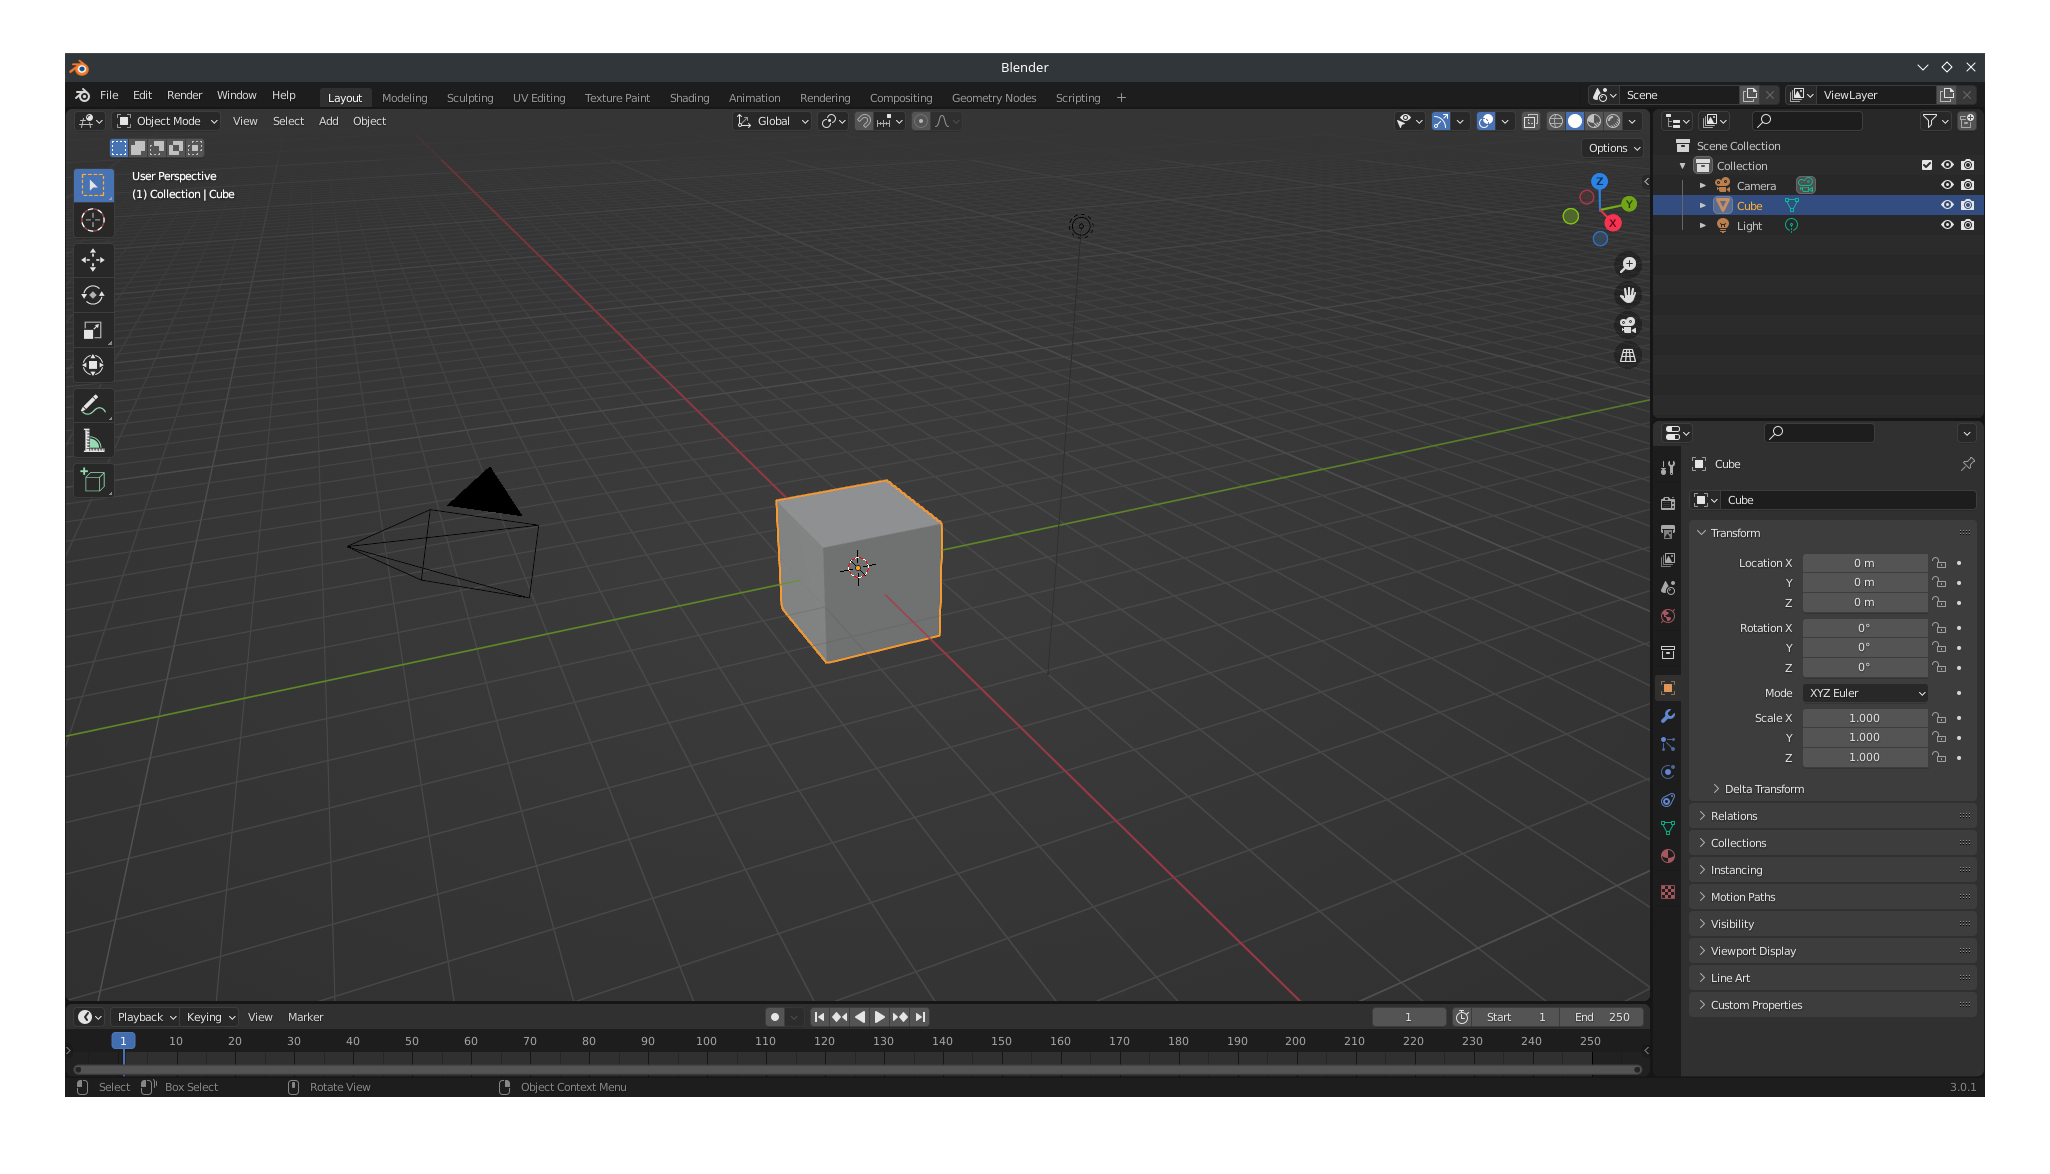
\includegraphics[width=0.9\textwidth]{images/blender.png}
	\caption{Interfejs programu Blender \cite{BLENDER} używanego do modelowania 3D}
	\label{blendermodel}
\end{figure}


\subsubsection{Formaty opisu sceny glTF}

Liczba możliwych elementów składającymi się na zasób 3D skłoniła branżę do opracowania ustandaryzowanych formatów opisu sceny, wśród których szczególną popularność zdobyły:
\begin{itemize}
	\item \textit{FBX} (Filmbox): rozwijany od 2006 przez Autodesk zamknięty format szeroko używany w branży gier z powodu łatwego eksportu oferowanego przez programy Autodesk 3ds Max i Maya.
	Jego zamknięta natura wymaga importowania albo przy pomocy oficjalnego SDK wymagającego akceptacji restrykcyjnego EULA, albo reimplementacji wymaganych części formatu inżynierią wsteczną.
	\item \textit{USD} (Universal Scene Description): otwarty format rozwijany od 2016 przez Pixar pozwala na łatwą i kompletną wymianę informacji pomiędzy różnymi najnowocześniejszymi programami grafiki 3D używanymi przez Pixar do produkcji animacji.
	Jego skompresowany i okrojony zamknięty wariant \textit{USDZ} jest używany przez Apple.
	\item \textit{glTF} (Graphics Language Transmission Format): rozwijany od 2015 przez Khronos otwarty format przystosowany do przechowywania ostatecznej wersji sceny w sposób prosty do sparsowania i wyrenderowania bądź dalszego przetworzenia.
	Wersja 2.0 wydana w 2021 zerwała kompatybilność wsteczną z wersją 1.0 i całkowicie ją zastąpiła.
\end{itemize}

Wśród wymienionych formatów jedynie glTF jest w pełni otwarty i łatwo importowany, dlatego jest on dobrym wyborem jako format zasobów 3D używanych przez silnik graficzny. Na przykład Godot \cite{godotengine} wspiera glTF jako główny i rekomendowany format opisy sceny.

Zgodnie ze specyfikacją glTF \cite{GLTFSPEC} zasób jest reprezentowany przez:
\begin{itemize}
	\item plik tekstowy \textit{*.gltf} w formacie JSON zawierający pełny opis sceny i jej poszczególnych elementów,
	\item pliki binarne \textit{*.bin} zawierający dane buforów zawierających geometrię bądź animacje,
	\item pliki obrazów \textit{*.png} i \textit{*.jpg} opisujące tekstury,
\end{itemize}
Pliki binarne i obrazy mogą być osadzone bezpośrednio w obiecie JSON używając kodowania Base64.
Możliwe jest też użycie binarnej wersji formatu glTF pozwalający na przechowywanie wszystkich danych w jednym binarnym pliku \textit{.glb}.

Zasób glTF składa się z obiektu JSON zawierającego metadane oraz osobne tablice dla każdego typu elementu zasobu.
Elementy mogą odnosić się do innych elementów używając ich indeksów w odpowiednich tablicach.
Relacje pomiędzy różnymi typami elementów zostały pokazana na poniższym diagramie:
\begin{figure}[H]
	\centering
	\begin{tikzpicture}[node distance=0.5cm]
		\tikzstyle{entity} = [rectangle, minimum width=2cm, minimum height=0.5cm,text centered, draw=black]
		\tikzstyle{refers} = [thick,->,>=stealth]
		
		\node (scene) [entity] {scene};
		\node (node) [entity, below = of scene] {node};
		\node (mesh) [entity, below = of node] {mesh};
		\node (accessor) [entity, below = of mesh] {accessor};
		\node (bufferView) [entity, below = of accessor] {bufferView};
		\node (buffer) [entity, below = of bufferView] {buffer};
		
		\node (camera) [entity, above right = of node] {camera};
		\node (skin) [entity, left = of node] {skin};
		\node (animation) [entity, below = of skin] {animation};
		
		\node (material) [entity, right = of accessor] {material};
		\node (texture) [entity, below = of material] {texture};
		\node (image) [entity, below = of texture] {image};
		\node (sampler) [entity, right = of image] {sampler};
		
		\draw [refers] (scene) edge[] (node);
		\draw [refers] (node) edge[] (mesh);
		\draw [refers] (mesh) edge[] (accessor);
		\draw [refers] (accessor) edge[] (bufferView);
		\draw [refers] (bufferView) edge[] (buffer);
		\draw [refers] (node) edge[out=-5,in=5, loop] (node);
		\draw [refers] (node) edge[] (camera);
		\draw [refers] (mesh) edge[] (material);
		\draw [refers] (material) edge[] (texture);
		\draw [refers] (texture) edge[] (image);
		\draw [refers] (texture) edge[] (sampler);
		\draw [refers] (node) edge[] (skin);
		\draw [refers] (skin) edge[] (node);
		\draw [refers] (skin) edge[out=-10,in=180,looseness=0] (accessor);
		\draw [refers] (animation) edge[] (node);
		\draw [refers] (animation) edge[] (accessor);
		
	\end{tikzpicture}
	\caption{Relacje pomiędzy rożnymi typami elementów w formacie glTF}
	\label{gltf_concepts}
\end{figure}

// TODO Opisz poszczególne typy elementów?

Przykładowo plik \textit{triangle.gltf} opisujący scenę zawierającą pojedyńczy trójkątą z geometrią składającą się z wierzchołków pozycji zawartych w pliku \textit{triangle.bin} wygląda następująco:

\noindent\begin{minipage}{.35\textwidth}
\lstset{language=JSON}
\begin{lstlisting}
{
  "asset" : {
    "version" : "2.0"
  },
  "scene" : 0,
  
  "scenes" : [
  {
    "nodes" : [ 0 ]
  } ],
  "nodes" : [
  {
    "mesh" : 0
  } ],
  "meshes" : [
  {
    "primitives" : [ {
      "attributes" : {
        "POSITION" : 0
      }
    } ]
  } ],
\end{lstlisting}
\end{minipage}\hfill
\begin{minipage}{.55\textwidth}
\lstset{language=JSON}
\begin{lstlisting}[frame=l]
  "buffers" : [
  {
    "uri" : "triangle.bin",
    "byteLength" : 36
  } ],
  "bufferViews" : [
  {
    "buffer" : 0,
    "byteOffset" : 0,
    "byteLength" : 36,
    "target" : 34962
  } ],
  "accessors" : [
  {
    "bufferView" : 0,
    "byteOffset" : 0,
    "componentType" : 5126,
    "count" : 3,
    "type" : "VEC3",
    "max" : [ 1.0, 1.0, 0.0 ],
    "min" : [ 0.0, 0.0, 0.0 ]
  } ]
}
\end{lstlisting}
\end{minipage}

\subsection{Zasoby wyjściowe}

Zasoby wyjściowe mają formę plików w formacie przystosowanym do manipulacji przez aplikację. Przykładami zasobów wyjściowych są pliki z rozszerzeniami \textit{.uasset} i \textit{.umap} używane przez silnik Unreal Engine \cite{unrealengine} do przechowywania zasobów w zoptymalizowanym formacie binarnym czy pliki \textit{.streamdb} i \textit{.resources}, które według twórców narzędzia do ekstrakcji zasobów z gier UnArch \cite{UNARCH} są używane w grze Doom Eternal i zastąpiły pliki \textit{.pak} wcześniejszych gier od id Software.


\subsection{Potok zasobów}

Potok zasobów (ang. asset pipeline) to część silnika odpowiadająca za konwersję zasobów wejściowych na zasoby wyjściowe.
Konwersja ta jest wymagana, ponieważ istnieją różne wymagania dotyczące formatów: zasoby wejściowe są zoptymalizowane pod kątem oszczędności miejsca na dysku i interoperacyjności między oprogramowaniem zewnętrznym, kiedy zasoby wyjściowe zwykle wymagają mniejszego zakresu możliwych funkcjonalności i powinny być w formacie dostosowanym do maksymalnie szybkiego wczytywania przez aplikację - szybkość ich zapisu jest mniej ważna ponieważ musi się odbyć tylko jeden raz na komputerach twórców oprogramowania uruchamiających potok zasobów.

\subsection{Baza zasobów}
Baza zasobów (ang. asset database) to zasób wyjściowy mający na celu zgromadzenie informacji o wszystkich zasobach używanych przez silnik.
// HIRO



// TODO

\section{Graf sceny}

Hierarchiczne modelowanie to technika reprezentowania złożonych obiektów polegająca na podzieleniu modelu na części i śledzeniu hierarchicznych relacji rodzic-dziecko pomiędzy nimi przy użyciu struktury zwanej grafem sceny.

Każdy węzeł grafu sceny składa się z lokalnej transformacji przestrzeni świata, opcjonalnej referencji do renderowanej geometrii oraz listy węzłów potomne.
Przemierzanie grafu pozwala na łatwe emitowanie poleceń rysowania:
// HIRO listing

// HIRO diagram graf sceny -> polecenia rysowania

Ten sposób reprezentacji sceny bardzo popularny wśród aplikacji 3D i jest używany przez formaty FBX i glTF.

// HIRO wydajność

\section{Graf renderowania}

// TODO
\chapter{Narzędzia, architektura i implementacja}
\label{chap:algs}

\section{Narzędzia}

Silnik została napisany jako biblioteka w języku C w standardzie C11. Budowanie biblioteki ze źródeł wymaga generacji
dodatkowego kodu przy pomocy skryptów w języku Python w wersji 3.9.7.

Silnik został w całości opracowany na przy użyciu środowiska programistycznego CLion w wersji 2021.2.3.

Proces testowania i debugowania odbywał się na maszynie o następującej konfiguracji:
\begin{itemize}
	\item {OS}: Kubuntu 22.04.1 LTS x86-64,
	\item {CPU}: 11th Gen Intel Core i5-11400 (2.60GHz),
	\item {GPU}: Intel UHD Graphics 730 (Rocket Lake GT1).
\end{itemize}

Podczas pracy stosowano rozproszony system kontroli wersji git. Repozytorium jest utrzymywane na serwisie GitHub.

Pliki \textit{.clang-tidy} i \textit{.clang-format} znajdujące się w strukturze plików projektu pozwalają na automatyczne formatowanie
kodu źródłowego zgodnie ze uprzednio zdefiniowanym standardem kodowania.

Proces budowania projektu jest zautomatyzowany przy użyciu narzędzia CMake, które w przypadku języków C i C++ jest
praktycznie standardem podczas rozwoju wieloplatformowych projektów.

\subsection{Proces budowania}

Proces budowania silnika jest zdefiniowany w pliku *CMakeLists.txt* znajdującym się w katalogu głównym projektu.

Kompilacja kodu źródłowego w języku C jest obsługiwana bezpośrednio przez CMake, które generuje standardowe pliki
kompilacji (pliki Makefile w systemie Unix, projekty Microsoft Visual C++ w systemie Windows). Użyto prekompilowanych
nagłówków do przyśpieszenia kompilacji bibliotek zewnętrznych.

Skrypty w języku Python są obsługiwane pośrednio przez CMake, które wykrywa zainstalowany interpreter języka Python i
używa go do stworzenia tzw. środowiska wirtualnego w tymczasowym katalogu venv/ w głównym katalogu projektu. Podczas
procesu budowania środowisko wirtualne jest używane do zainstalowania wymaganych zewnętrznych bibliotek w języku Python
i wykonywania skryptów generatora kodu. Zaletą użycia środowiska wirtualnego w porównaniu do bezpośredniego wywoływania
zainstalowanego interpretera Pythona jest izolacja zarządzania zależnościami od reszty systemu operacyjnego, co pozwala
na łatwiejszą powtarzalność podczas debugowania \cite{PEP405}.

CMake organizuje proces budowania jako graf, w którym wierzchołki to cele połączonych ze sobą zależnościami. Budowa celu
wymaga wcześniejszego zbudowania wszystkich innych celów od których zależy budowany cel.

Wyróżniane są trzy rodzaje celów:
\begin{itemize}
	\item {plik wykonywalny}
	\item {biblioteka}: statyczna lub dynamiczna
	\item {cel niestandardowy}: używany do uruchamiania zewnętrznych programów podczas procesu kompilacji, np. generatorów kodu
\end{itemize}

Poniższy diagram przedstawia proces budowania projektu w formie celów i ich zależności:
\begin{figure}[H]
	\centering
	\begin{tikzpicture}[node distance=2cm]
		\tikzstyle{module} = [rectangle, rounded corners, minimum width=3cm, minimum height=1cm,text centered, draw=black]
		\tikzstyle{arrow} = [thick,->,>=stealth]
		
		\node (main) [module] {main};
		\node (test) [module, right = of main] {test};
		\node (assetpipeline) [module, right = of test] {asset\_pipeline};
		
		\node (engine) [module, below = of main] {engine};
		
		\node (runassetpipeline) [module, above = of assetpipeline] {run\_asset\_pipeline};
		\node (copyasset) [module, left = of runassetpipeline] {copy\_asset};
		
		\draw [arrow] (main) -- (engine);
		\draw [arrow] (test) edge[out=180, in=45] (engine);
		\draw [arrow] (assetpipeline) edge[out=-90, in=0] (engine);
		
		\draw [arrow] (main) edge[]  (runassetpipeline);
		\draw [arrow] (test) edge[]  (runassetpipeline);
		
		\draw [arrow] (runassetpipeline) -- (assetpipeline);
		
		\draw [arrow] (main) -- (copyasset);
		\draw [arrow] (test) -- (copyasset);
		\draw [arrow] (assetpipeline) -- (copyasset);
		\draw [arrow] (runassetpipeline) -- (copyasset);
		
		\node(plikiwykonywalne)[draw,dotted,fit=(main) (test) (assetpipeline)] {};
		\node (plikiwykonywalneLabel)[below=0cm of plikiwykonywalne] {\textbf{Pliki wykonywalne}};
		
		\node(biblioteki)[draw,dotted,fit=(engine)] {};
		\node (bibliotekiLabel)[below=0cm of biblioteki] {\textbf{Biblioteki}};
		
		\node(celeniestandardowe)[draw,dotted,fit=(copyasset) (runassetpipeline)] {};
		\node (celeniestandardoweLabel)[above=0cm of celeniestandardowe] {\textbf{Cele niestandardowe}};
		
	\end{tikzpicture}
	\caption{Proces budowania w formie celów i ich zależności (opracowanie własne)}
	\label{cmake}
\end{figure}

\paragraph{engine} Cel budujący bibliotekę programistyczną zawierającą implementację silnika.

\paragraph{main} Cel budujący plik wykonywalny demonstujący użycie silnika poprzez wyrenderowanie przykładowej sceny.

\paragraph{test} Cel budujący plik wykonywalny z testami jednostkowymi napisanymi i używanymi podczas implementowania projektu.

\paragraph{asset\_pipeline} Cel budujący plik wykonywalny służący jako narzędzie wiersza poleceń wykonujące operacje potoku zasobów.

\paragraph{copy\_assets} Niestandardowy cel kopiujący podkatalogu głównego \textit{assets} zawierającego nieprzetworzone zasoby wejściowe do katalogu budowania.

\paragraph{run\_asset\_pipeline} Niestandardowy cel realizujący potoku zasobów poprzez uruchomienie skryptu Python wielokrotne uruchamiającego narzędzie \textbf{asset\_pipeline} na zasobach wejściowych.


\subsection{Biblioteki zewnętrzne}

Projekt używa następujących zewnętrznych bibliotek programistycznych:

\begin{itemize}
	\item {\textit{Vulkan SDK 1.3.211.0}}:
	\begin{itemize}
		\item pliki nagłówkowe dla Vulkan,
		\item \textit{shaderc}: kompilacja shaderów z kodu źródłowego GLSL do kodu bajtowego SPIR,
		\item \textit{SPIRV-Reflect}: mechanizm refleksji dla kodu bajtowego SPIR-V,
	\end{itemize}
	\item {\textit{glfw 3.4}}: międzyplatformowa obsługa tworzenia okien, obsługa wejścia klawiatury i myszy,
	\item {\textit{sqlite 3.35.5}}: relacyjna baza danych SQL,
	\item {\textit{uthash 2.3.0}}: proste struktury danych (tablica dynamiczna, lista dwukierunkowa, tablica mieszająca),
	\item {\textit{xxHash 0.8.1}}: niekryptograficzny algorytm mieszający,
	\item {\textit{cgltf 1.11}}: wczytywanie plików w formacie glTF,
	\item {\textit{cglm 0.8.5}}: biblioteka matematyczna,
	\item {\textit{stb\_image 2.27}}: wczytywanie obrazów,
	\item {\textit{stb\_truetype 1.26}}: rasteryzacja tekstu czcionek,
	\item {biblioteka standardowa języka C},
	\item {API systemu operacyjnego}: pliki nagłówkowe POSIX albo WinAPI,
	\item {biblioteka standardowa języka Python},
	\item {\textit{libclang 12.0.0}}: analizowanie kodu C w skryptach Python.
\end{itemize}

Dodatkowo biblioteka zbudowana w konfiguracji \textit{Debug} statycznie linkuje biblioteki \textit{ASan} (AddressSanitizer) i \textit{UBSan} (
UndefinedBehaviorSanitizer) wykrywające szeroką klasę błędów dotyczących niewłaściwego użycia pamięci i niezdefiniowanych zachowań. Błędy te w języku C są nieoczywiste i trudne do wykrycia przez programistę. Podczas rozwoju projektu ASan wielokrotnie pozwolił na wykrycie i naprawienie następujących rodzajów błędów:

\begin{itemize}
	\item wycieki pamięci,
	\item dereferencje zwisających wskaźników,
	\item dereferencja wskaźników NULL,
	\item dereferencja źle wyrównanych struktur,
	\item odczyt i zapis poza granicami tablicy.
\end{itemize}

\section{Architektura}

Silnik jest zaprojektowany w duchu architektury modułowej - funkcjonalność biblioteki jest rozdzielona na bloki zwane modułami, które mogą być rozwijane niezależnie od pozostałych modułów.

Silnik był rozwijany metodą \textit{bottom-up} - jego pierwsza iteracja była pojedynczym plikiem źródłowym wyświetlającym trójkąt \cite{VULKANTUTORIAL}, który w procesie dekompozycji i refaktoryzacji organicznie rozrósł się do 7 modułów znajdujących się w osobnych podkatalogach zawierających łącznie 9 skryptów Python \textit{.py}, 65 nagłówków \textit{*.h} i 63 plików źródłowych \textit{*.c}.

Obecnie silnik składa się z następujących modułów:
// TODO lista modułów, podkatalog i przeznaczenie

Moduł jest dalej podzielony na jednostki, które zostały na potrzeby projektu zdefiniowane jako para składająca się z pliku nagłówkowego z odpowiadającym plikiem źródłowymi o tej samej nazwie.

Pliki nagłówowe zawierają deklaracje funkcji, struktur oraz typów wyliczeniowych widocznych dla użytkownika końcowego i powinny być dołączone do programu przy użyciu dyrektywy \textit{\#include} preprocesora.
Pliki źródłowe zawierają definicje deklaracji plika nagłówkowego i powinny być dołączone do programu używając argumentów kompilatora (jeśli dodawane są niezbudowane pliki źródłowe) bądź linkera (jeśli dodawane są zbudowane pliki biblioteczne), co jest automatycznie wykonywane przez CMake.

Struktury są zorganizowane w sposób obiektowy.
Język C nie posiada wbudowanej koncepcji klasy, ale w projekcie przyjęto założenie, że dla klasy \textit{struct} jej stan jest reprezentowany przez strukturę \textit{struct}, która może posiadać metodę \textit{func()}, jeśli istnieje funkcja \textit{struct\_func()} przyjmująca wskaźnik do \textit{struct} jako pierwszy argument.
Dla obiektów globalnych nie jest istnieje osobna struktura przekazywana do jej metod - stan obiektu jest zaszyty w zmiennych globalnych jednostki translacji pliku źródłowego.

Obiekty mogą oferować metody \textit{create()} i \textit{destroy()}, które alokują lub dealokują instancję obiektu oraz tworzą bądź niszczą jej wewnętrzny stan.
Analogiczne metody \textit{init()} i \textit{deinit()} tworzą i niszczą instancję, której pamięć została wcześniej zaalokowaną (np. na stosie lub w tablicy).
Opcjonalna metoda \textit{debug\_print()} loguje informacje o wewnętrznym stanie instancji użyteczne podczas debugowania.

Relacje pomiędzy modułami silnika i ich najważniejszymi jednostkami są przedstawione na poniższym diagramie:

// TODO: Ładniejszy diagram, relacje.
\begin{figure}[H]
	\centering
	\begin{tikzpicture}[node distance=2mm]
		\tikzstyle{class} = [rectangle, minimum width=2cm, minimum height=5mm,text centered, draw=black]
		\tikzstyle{file} = [rectangle, minimum width=2cm, minimum height=5mm,text centered, draw=gray]
		\tikzstyle{file2} = [file, minimum width=3cm]
		\tikzstyle{executable} = [rectangle, rounded corners, minimum width=1cm, minimum height=5mm,text centered, draw=gray]

		\tikzstyle{arrow} = [thick,->,>=stealth]
		\tikzstyle{relation} = [densely dotted]
		
		% codegen
		\node (descriptors) [file] {descriptors};
		\node (constants) [file, below = of descriptors] {constants};
		\node (globals) [file, below = of constants] {globals};
		\node (macros) [file, below = of globals] {macros};
		\node (meta) [file, below = of macros] {meta};
		\node(codegen)[draw,dotted,fit=(descriptors) (meta)] {};
		
		% core
		\node (alloc) [file, below = 1cm of codegen] {alloc};
		\node (junk) [file, below = of alloc] {junk};
		\node (log) [file, below = of junk] {log};
		\node (platform) [file, below = of log] {platform};
		\node (thirdparty) [file, below = of platform] {thirdparty};
		\node(core)[draw,dotted,fit=(alloc) (junk) (log) (platform) (thirdparty)] {};
		
		% data
		\node (db) [file, below = 1cm of core] {sql\_db};
		\node (config) [file, below = of db] {config};
		\node (assetdb) [file, below = of config] {asset\_db};
		\node(data)[draw,dotted,fit=(db) (assetdb)] {};
		
		% assets
		\node (assetcommon) [file2, right = 1cm of db] {asset\_common}; \def\y{assetcommon};
		\def\x{asset_camera}; \node (\x) [file2, below = of \y] {\myesc{\x}}; \edef\y{\x};
		\def\x{asset_direct_light}; \node (\x) [file2, below = of \y] {\myesc{\x}}; \edef\y{\x};
		\def\x{asset_material}; \node (\x) [file2, below = of \y] {\myesc{\x}}; \edef\y{\x};
		\def\x{asset_vertex_attribute}; \node (\x) [file2, right = of assetcommon] {\myesc{\x}}; \edef\y{\x};
		\def\x{asset_primitive}; \node (\x) [file2, below = of \y] {\myesc{\x}}; \edef\y{\x};
		\def\x{asset_mesh}; \node (\x) [file2, below = of \y] {\myesc{\x}}; \edef\y{\x};
		\def\x{asset_object}; \node (\x) [file2, below = of \y] {\myesc{\x}}; \edef\y{\x};
		\def\x{asset_image}; \node (\x) [file2, right = of asset_vertex_attribute] {\myesc{\x}}; \edef\y{\x};
		\def\x{asset_sampler}; \node (\x) [file2, below = of \y] {\myesc{\x}}; \edef\y{\x};
		\def\x{asset_texture}; \node (\x) [file2, below = of \y] {\myesc{\x}}; \edef\y{\x};
		\def\x{asset_skybox}; \node (\x) [file2, below = of \y] {\myesc{\x}}; \edef\y{\x};
		\def\x{asset_font}; \node (\x) [file2, below = of \y] {\myesc{\x}}; \edef\y{\x};
		\node (assetpipeline) [executable, below = of asset_object] {asset\_pipeline};
		\node(assets)[draw,dotted,fit=(assetcommon) (asset_font)] {};
	
		% scene
		\node (scene_data) [file, right = 1cm of thirdparty] {scene\_data}; \def\y{scene_data};
		\def\x{scene_graph}; \node (\x) [file, right = of \y] {\myesc{\x}}; \edef\y{\x};
		\def\x{scene_tree}; \node (\x) [file, right = of \y] {\myesc{\x}}; \edef\y{\x};
		\node(scene)[draw,dotted,fit=(scene_data) (scene_tree)] {};
		
		% objects
		\node (buffer) [file, right = 2cm of descriptors] {buffer}; \def\y{buffer};
		\def\x{image}; \node (\x) [file, below = of \y] {\myesc{\x}}; \edef\y{\x};
		\def\x{vertex_stream};\node (\x) [file, below = of \y] {\myesc{\x}}; \edef\y{\x};
		\def\x{device}; \node (\x) [file, right = 1cm of buffer] {\myesc{\x}}; \edef\y{\x};
		\def\x{swap_chain}; \node (\x) [file, below = of \y] {\myesc{\x}}; \edef\y{\x};
		\def\x{sync}; \node (\x) [file, below = of \y] {\myesc{\x}}; \edef\y{\x};
		\def\x{unified_uniform_buffer}; \node (\x) [file, below = 4mm of vertex_stream] {\myesc{\x}}; \edef\y{\x};
		\def\x{textures}; \node (\x) [file, below = of \y] {\myesc{\x}}; \edef\y{\x};
		\def\x{unified_geometry_buffer}; \node (\x) [file, below = of \y] {\myesc{\x}}; \edef\y{\x};
		\def\x{descriptors};\node (\x) [file, right = 4mm of unified_uniform_buffer] {\myesc{\x}}; \edef\y{\x};
		\def\x{shader};\node (\x) [file, below = of \y] {\myesc{\x}}; \edef\y{\x};
		\node(objects)[draw,dotted,fit=(device) (unified_geometry_buffer) (shader)] {};
		
		% renderer
		\node (renderer) [file, right = 1cm of device] {renderer}; \def\y{renderer};
		\def\x{render_state}; \node (\x) [file, below = of \y] {\myesc{\x}}; \edef\y{\x};
		\def\x{renderer_cache}; \node (\x) [file, below = of \y] {\myesc{\x}}; \edef\y{\x};
		\def\x{render_graph}; \node (\x) [file, right = of renderer] {\myesc{\x}}; \edef\y{\x};
		\def\x{render_pass}; \node (\x) [file, below = of \y] {\myesc{\x}}; \edef\y{\x};
		\def\x{render_pass_state}; \node (\x) [file, below = of \y] {\myesc{\x}}; \edef\y{\x};
		\def\x{batch}; \node (\x) [file, below = of \y] {\myesc{\x}}; \edef\y{\x};
		\def\x{main}; \node (\x) [executable, below = of \y] {\myesc{\x}}; \edef\y{\x};
		\node(rendering)[draw,dotted,fit=(renderer) (renderer_cache) (render_pass_state) (main)] {};
	
		% labels
		\node ()[above=0cm of codegen] {\textbf{Wygenerowany kod}};
		\node ()[above=0cm of core] {\textbf{Rdzeń}};
		\node ()[above=0cm of data] {\textbf{I/O}};
		\node ()[below=0cm of assets] {\textbf{Zasoby}};
		\node ()[above=0cm of objects] {\textbf{Vulkan}};
		\node ()[below=0cm of scene] {\textbf{Scena}};
		\node ()[above=0cm of rendering] {\textbf{Renderer}};
		
	\end{tikzpicture}
	\caption{Relacje pomiędzy modułam silnika i ich najważniejszymi klasami (opracowanie własne)}
	\label{archit}
\end{figure}

\section {Implementacja}

Ta sekcja opisuje szczegóły implementacyjne poszczególnych modułów silnika.

\subsection{Wygenerowany kod}

Silnik używa kodu w języku C wygenerowanego przez automatyczny generator kodu będący skryptem Python uruchamianym przez CMake na początku procesu budowania przed rozpoczęciem kompilacji właściwego
kodu źródłowego biblioteki.

Język C nie posiada mechanizmów pozwalających na metaprogramowanie z wyjątkiem makr preprocessora, które mogą zaspokoić część potrzeb programisty chcącego przykładowo dodać nowy rodzaje pętli \cite{METACONTROLC}, ale nie pozwalają na bardziej skomplikowaną analizę i przekształcanie kodu, które muszą być wykonywane przez zewnętrzne narzędzia.

Działanie skryptu jest sterowane konfiguracją generatora, który jest plikiem w formacie INI (zgodnym z biblioteką \textit{configparser} \cite{PYTHONCONFIGPARSER}) znajdującym się w katalogu ze skryptem.
Format INI nie posiada standardowej specyfikacji, ale tradycyjnie jest on plikiem tekstowym podzielonym na sekcje zawierające pary klucz-wartość.

Skrypt parsuje pliki nagłówkowe języka C znajdujący się w katalogu /src z
pominięciem katalogu /src/codegen, do którego skrypt zapisuje wygenerowane pliki nagłówkowe i źródłowe, które są kolejno dołączane w innych modułach silnika i dodawane jako argumenty kompilatora.
Razem wszystkie wygenerowane pliki tworzą jednostki modułu wygenerowanego kodu.


\subsubsection{Jednostka constants}
Zawiera wygenerowane stałe: wartości zdefiniowane w sekcji \textit{CONSTANTS} konfiguracji generatora używane przez resztę modułów, które zostały uznane za zbyt niepraktyczne aby pozwolić na ich modyfikację przy użyciu konfiguracji globalnej.
Poniżej wymieniono stałe, ich wartości oraz interpretacje:
\begin{itemize}
	\item \textit{FRAMES\_IN\_FLIGHT}: $2$, liczba klatek "w locie" (ang. in flight frames), czyli jednocześnie renderowanych przez GPU, domyślna wartość pozwala na podwójne buforowanie; 
	\item \textit{MAX\_OFFSCREEN\_TEXTURE\_COUNT}: $16$, maksymalna liczbę tekstur pozaekranowych;
	\item \textit{MAX\_RENDER\_TARGET\_COUNT}: $8$, maksymalną liczbę tekstur pozaekranowych, które mogą być używane jako cele renderowania podczas jednego przebiegu; 
	\item \textit{MAX\_FRAMEBUFFER\_ATTACHMENT\_COUNT}: \textit{MAX\_RENDER\_TARGET\_COUNT + 1 + 1}, maksymalna liczba dołączeń używana przez potok graficzny - wystarcza na dołączenia celów renderowania, prezentowalnego obrazu i bufor głębi;
	\item \textit{MAX\_INDIRECT\_DRAW\_COMMAND\_COUNT}: $1024$, maksymalna liczba poleceń rysowania które mogą być wykonana przez jedno polecenie rysowania pośredniego;
	\item \textit{MAX\_MATERIAL\_COUNT}: $128$, maksymalna liczba materiałów;
	\item \textit{MAX\_DIRECTIONAL\_LIGHT\_COUNT}: $1$, maksymalna liczbę świateł kierunkowych na scenie;
	\item \textit{MAX\_POINT\_LIGHT\_COUNT}: $128$, maksymalna liczbę świateł punktowych na scenie;
	\item \textit{MAX\_TEXT\_CHARACTER\_COUNT}: $256$, maksymalną liczbę znaków w renderowanym ciągu znaków;
	\item \textit{MIN\_DELTA\_TIME}: $(1.0 / 30.0)$, minimalny czas pomiędzy wywołaniami funkcji zwrotnej \textit{update} w pętli głównej, domyślnie $\frac{1}{30}$ sekundy (30 FPS);
	\item \textit{WORLD\_UP}: $0, 1, 0$; wektor interpretowany jako "w górę" w przestrzeni świata.
\end{itemize}

Wygenerowane stałe mogą być używane przez shadery - ich definicje są umieszczane na początku kodu GLSL shadera przed jego kompilacją - dlatego są one udostępiane w formie X makro \textit{CODEGEN\_CONSTANTS}.

X makro to przydatna technika preprocessora pozwalająca na pisanie kodu, który jest automatycznie aktualizowany po zmienie danych opisywanych przez X makro \cite{XMACRO}.
Przykładowo poniższa funkcja wymaga manualnej aktualizacji po zmianie używanego typu wyliczeniowego:
\lstset{language=C}
\begin{lstlisting}[caption={Przykładowy kod przed zastosowaniem X makro},captionpos=b]
typedef enum key {
	key_space,
	key_enter,
	key_count,
} key;

int key_to_glfw_key(key value) {
	switch (value) {
		case key_space: return GLFW_KEY_SPACE;
		case key_enter: return GLFW_KEY_ENTER;
		default: return GLFW_KEY_UNKNOWN;
	}
}
\end{lstlisting}
Ten sam kod używający X makro:
\lstset{language=C}
\begin{lstlisting}[caption={Przykładowy kod po zastosowaniu X makro},captionpos=b]

#define END_OF_KEYS
#define KEYS(X, ...)			\
	X(space, GLFW_KEY_SPACE)	\
	X(enter, GLFW_KEY_ENTER)	\
	END_OF_KEYS

typedef enum key {
#define x(_name, ...) key_##_name,
	KEYS(x, )
#undef x
	key_count,
} key;

int key_to_glfw_key(key value) {
	switch (value) {
#define x(_name, _value, ...) case key_##_name: return _value;
		KEYS(x, )
#undef x
		default: return GLFW_KEY_UNKNOWN;
	}
}
\end{lstlisting}
X makra ułatwiają utrzymywanie kodu poprzez deklaratywnego "jedynego źródła prawdy"\  i są intensywnie używane na wskroś silnika.

\subsubsection{Jednostka globals}
Obiekt globalny \textit{globals} reprezentujący wygenerowane zmienne.
Ich wartości, w przeciwieństwie stałych, mogą być ustalone dopiero w czasie wykonywania.
Obiekt jest używany do specyfikacji struktury różnych ścieżek katalogów i plików używanych przez silnik.

Silnik używa poniższej sekcji konfiguracji generacji do opisania ścieżkek dla kolejno katalogu zasobów, konfiguracji globalnej, bazy zasobów, katalogu shaderów i ich współdzielonego kodu GLSL oraz pliku logowania:
\lstset{language=verbatim}
\begin{lstlisting}[caption={Konfiguracja generacji zmiennych},captionpos=b]
[GLOBALS]
assetsDirname = assets
assetDatabaseFilepath = ${assetsDirname}/data.db
assetConfigFilepath = ${assetsDirname}/config.ini
assetsShaderDirpath = ${assetsDirname}/shaders
assetsShaderCommonFilepath = ${assetsShaderDirpath}/common.glsl
logFileName = log.txt
\end{lstlisting}
Powyższa konfiguracja generuje poniższą metodę init():
\lstset{language=C}
\begin{lstlisting}[caption={Wynik generacji zmiennych},captionpos=b]
void globals_create() {
	globals.assetsDirname =
		get_executable_dir_file_path("", "assets");
	globals.assetDatabaseFilepath =
		get_executable_dir_file_path("", "assets/data.db");
	globals.assetConfigFilepath =
		get_executable_dir_file_path("", "assets/config.ini");
	globals.assetsShaderDirpath =
		get_executable_dir_file_path("", "assets/shaders");
	globals.assetsShaderCommonFilepath =
  		get_executable_dir_file_path("", "assets/shaders/common.glsl");
	globals.logFileName =
		get_executable_dir_file_path("", "log.txt");
}
\end{lstlisting}

\subsubsection{Jednostka macros}
Zbiór X makr używanych przez moduł I/O obsługujący następujące zasoby wejściowe.

Makra opisują wewnętrzną strukturę plików INI konfiguracji globalnej i konfiguracji zasobów: używane sekcje i ich dopuszczalne pary klucz-wartość z domyślnymi wartościami (liczby całkowite bądź ciągi znaków).
Przykładowy fragment konfiguracji generatora opisujący konfiguracji globalnej:
\lstset{language=verbatim}
\begin{lstlisting}[caption={Konfiguracja generacji konfiguracji globalnej},captionpos=b]
[GLOBAL.CONFIG]
graphics.WindowWidth = 640
controls.Enabled = 1
settings.StartScene = "sponza"
\end{lstlisting}
Powyższa konfiguracja pozwala silnikowi na sparsowanie poniższego pliku INI:
\lstset{language=verbatim}
\begin{lstlisting}[caption={Przykładowa konfiguracja globalna},captionpos=b]
[settings]
StartScene = MetalRoughSpheresNoTextures

[graphics]
WindowWidth = 1024

[controls]
Enabled = 1 
\end{lstlisting}

Podobnie opisywana jest struktura bazy zasobów: typy podstawowe i ich odpowiedniki w języku C oraz tabele i ich kolumny. Ilustruje to poniższy fragment konfiguracji generatora:
\lstset{language=verbatim}
\begin{lstlisting}[caption={Fragment konfiguracji generatora opisujący strukturę bazy zasobów},captionpos=b]
[ASSET.DB]
types = "BYTE:uint8_t, INT:uint32_t, FLOAT:float, TEXT:UT_string *, KEY:hash_t"
image = "key KEY, width INT, height INT, depth INT, channels INT, type INT, data BYTE_ARRAY"
sampler = "key KEY, magFilter INT, minFilter INT, addressWrapU INT, addressWrapV INT"
texture = "key KEY, image KEY, sampler KEY"
\end{lstlisting}

Struktura zasobów wejściowych zostanie dokładniej opisana w dalszym podrozdziale o module I/O.

\subsubsection{Jednostka meta}
Funkcje pomocnicze wygenerowane na podstawie nagłówków silnika i Vulkan SDK.

Dla każdego napotkanego typu wyliczeniowego \textit{EnumName} jest generowana jedna z poniższych funkcji:
\lstset{language=C}
\begin{lstlisting}[caption={Wygenerowane funkcje dla typów wyliczeniowych},captionpos=b]
const char *EnumName_debug_str(int value);
void EnumName_debug_print(int flags, int indent);
\end{lstlisting}
Funkcje pozwalające na konwersję liczby całkowitej będącej wartoścą zmiennej wyliczeniowego na ciąg znaków i są używane przez metody \textit{debug\_print()} do logowania wartości w formie przyjaźniejszej dla użytkownika.

Funkcja \textit{*\_debug\_str()} jest generowana tylko wtedy, jeśli literały wyliczeniowe nie są flagami, tj. nie są kolejnymi potęgami liczby 2.


\subsubsection{Jednostka descriptors}
Jednostka zawierająca struktury i funkcje upraszczające pracę z deskryptorami.

Nagłówek \textit{descriptor} modułu Vulkan zawiera definicje struktur języka C opisujących wewnętrzną strukturę pamięci buforów i stałych push znajdujących się na GPU.
W zależności od nazwy dzielą się one na 3 rodziny:
\begin{itemize}
	\item \textit{*\_push\_constant\_struct}: stała push o nazwie \textit{*},
	\item \textit{*\_uniform\_buffer\_struct}: bufor uniform o nazwie \textit{*},
	\item \textit{*\_helper\_struct}: struktura pomocnicza o nazwie \textit{*} używana w powyższych.
\end{itemize}
Przykłady powyższych struktur:
\lstset{language=C}
\begin{lstlisting}[caption={Przykładowe struktury w nagłówku descriptor opisujące wewnętrzną strukturę deskryptorów},captionpos=b]
// stała push 'draw'
typedef struct draw_push_constant_struct {
	uint currentFrameInFlight;
} draw_push_constant_struct;

// struktura pomocnicza 'offscreen_texture'
typedef struct offscreen_texture_helper_struct {
	uint textureId; ///< array=MAX_OFFSCREEN_TEXTURE_COUNT
} offscreen_texture_helper_struct;

// stała push 'global'
typedef struct global_uniform_buffer_struct {
	mat4 viewMat;
	mat4 projMat;
	...
	offscreen_texture_helper_struct offscreenTextures;
} global_uniform_buffer_struct;
\end{lstlisting}

Układ pamięci struktur zdefiniowanych w języku C nie są koniecznie kompatybilne układem pamięci wymaganymi przez GPU.
Dlatego dla każdej sparsowanej struktury \textit{*\_struct} jest generowana analogiczna struktura \textit{*\_element}, w których użyto specyfikatorów \textit{alignas} i atrybutów \textit{packed} udostępnianych przez C11 i rozszerzenia GCC w celu wyrównania pól struktury w zgodzie ze standardem układu pamięci *scalar*.
Generowana jest też funkcja \textit{glsl\_add\_*()} dodająca do ciągu znaków z kodem GLSL definicje struktury i kwalifikator układu.
Przykładowe wejście i wyjście generacji dla bufora uniform \textit{instances}:
\lstset{language=C}
\begin{lstlisting}[caption={Przykładowe wejście i wyjście generacji dla bufora uniform},captionpos=b]
// descriptor.h:
typedef struct instances_uniform_buffer_struct {
	mat4 modelMat;
	uint materialId;
} instances_uniform_buffer_struct;
	
// descriptors.h
typedef struct PACKED_STRUCT instances_uniform_buffer_element {
	alignas(4) mat4 modelMat ;
	alignas(4) uint materialId ;
} instances_uniform_buffer_element;
void glsl_add_instances_uniform_buffer(
	UT_string *s, uint32_t set, uint32_t binding, uint32_t count);

// descriptors.c
void glsl_add_instances_uniform_buffer(
	UT_string *s, uint32_t set, uint32_t binding, uint32_t count) {
	utstring_printf(s, "struct instancesStruct {\n");
	utstring_printf(s, "  mat4 modelMat ;\n");
	utstring_printf(s, "  uint materialId ;\n");
	utstring_printf(s, "};\n");
	utstring_printf(s, "layout(scalar, set = %u, binding = %u) "
			   "uniform instancesBlock {\n", set, binding);
	utstring_printf(s, "  instancesStruct instances");
	if (count > 1) {utstring_printf(s, "[%u]", count);}
	utstring_printf(s, ";\n};\n");
}
\end{lstlisting}
Generacja jest kończona X makraami wyliczającymi nazwy wszystkich sparsowanych rodzin struktur. 

Dzięki automatycznej generacji kodu modyfikacja sposobu organizacji pamięci GPU buforów sprowadza się do modyfikacji struktur w nagłówku \textit{descriptors}, co pozwala na szybkie testowanie nowych parametrów i metod dostępu do nich podczas pisania shaderów.
Mechanizm ten został zainspirowany implementacją jednolitych buforów w grze \textit{Tom Clancy's Rainbow Six Siege} \cite{RAINBOWSIXSIEGE}.

Wygenerowane struktury, funkcje i X makra są używane podczas kopiowania danych z CPU do pamięci GPU oraz generacji shaderów, co zostanie dokładniej opisane w dalszym podrozdziale o module Vulkan.

\subsection{Rdzeń}

Rdzeń to moduł zawierający funkcje pomocniczych i obiekty globalne zapewniające podstawowe funkcjonalności używane przez resztę modułów.

\subsubsection{Jednostka thirdparty}
Jednostka odpowiedzialna za udostępnienia bibliotek zewnętrznych reszcie kodu.

Nagłówek dołącza nagłówki bibliotek zewnętrznych i z powodów wydajnościowych podczas procesu budowania jest traktowany jako nagłówek prekompilowany (ang. precompiled header, PCH).

Plik źródłowy obsługuje część bibliotek zewnętrznych składających się jedynie z nagłówków (ang. header-only library).
W przeciwieństwie do tradycyjnych bibliotek języka C w których kod jest podzielony na pliki nagłówkowe i źródłowe, w tym przypadku dostęp do definicji tradycyjnie znajdujących sę z plikach źródłowych jest uzyskiwany poprzez ponowne dołączenie nagłówka przy użyciu dyrektywy \textit{\#include} po wcześniejszym zdefiniowaniu odpowiedniego symbolu preprocesora.
Przykładowo biblioteka \textit{cgltf} wymaga ponownego dołączenia nagłówka w następujący sposób:
\lstset{language=C}
\begin{lstlisting}[caption={Przykład dołączenia implementacji bibliteki \textit{cgltf}},captionpos=b]
#define CGLTF_IMPLEMENTATION
#include "cgltf.h"
\end{lstlisting}

\subsubsection{Jednostka alloc}
Funkcje pomocnicze wspomagające zarządzanie pamięcią CPU, co objemuje alokację, dealokację, kopiowanie, duplikowanie i porównywanie bloków pamięci CPU.

Funkcje te są potrzebne, ponieważ działanie odpowiednich funkcji oferowane przez bibliotekę standardową języka C, chociaż oferują żądaną funkcjonalność, opiera się na mechanizmie niezdefiniowanych zachowań (ang. undefined behaviour) dla niektórych argumentów (wskaźnik NULL, rozmiar 0) i zachowań OOM (ang. Out-of-memory).

Funkcje pomocnicze są wrapperami z dodatkowymi instrukcjami warunkowymi sprawdzającymi, czy wywołanie funkcji nie skutkuje niezdefiniowanym zachowaniem.

Jednostka definiuje też makra ułatwiające zarządzanie pamięcią struktur danych bibliteki \textit{uthash}.


\subsubsection{Jednostka log}
Obiekt globalny \textit{log} reprezentujący system logowana komunikatów wygenerowanych podczas działania kodu mający na celu w uproszczenie procesu debuggowania.

Komunikat jest ciągiem znaków z przypisanym poziomem logowania określającym jego ważność z domyślnie wspieranymi wartościami \textit{debug}, \textit{info}, \textit{warn}, \textit{error} i \textit{fatal}.
Komunikaty \textit{debug} są logowane tylko w konfiguracji \textit{Debug}.

Komunikaty są zapisywane do standardowego wyjścia (\textit{stdout} albo \textit{stderr}) oraz do pliku tekstowego na dysku, którego nazwa zaostała zdefiniowana w wygenrowanych zmiennych (domyślnie \textit{log.txt}).

Logowanie komuniaktu odbywa się poprzez grupę funkcji \textit{log\_*()}, gdzie \textit{*} to poziom logowania, zachowujące się tak samo jak funkcja \textit{printf} z biblioteki standardowej języka C - pierwszy argument to ciąg znaków z znakami formatującymi, reszta argumentów to formatowane wartości.

Przykładowy kod demonstrujący logowanie:
\lstset{language=C}
\begin{lstlisting}[caption={Demonstracja logowania},captionpos=b]
log_create();
log_debug("komunikat #%d", 1);
log_debug("komunikat #%d", 2);
log_fatal("%s #%d", "komunikat", 3);
log_destroy();
\end{lstlisting}

Powyższy kod powinien zapisać do pliku \textit{log.txt} w katalogu z plikiem wykonywalnym komunikaty podobne do poniższych:
\lstset{language=verbatim}
\begin{lstlisting}[caption={Wynik logowania},captionpos=b]
[DEBUG] (/home/user/repo/src/main.c:45) main:
komunikat #1
komunikat #2
[FATAL] (/home/user/repo/src/main.c:47) main:
komunikat #3
\end{lstlisting}

\subsubsection{Jednostka junk}
Proste funkcje i makra które mogą być potencjalnie używane we wszystkich modułach bibliteki, ale nie zostały uznane za wystarczająca skomplikowane, aby uzasadnić wydzielenia do osobnej jednostki.

Jednostka definiuje stałe preprocesora \textit{PLATFORM\_*} używane do rozpoznania systemu operacyjnego, na którym budowany jest silnik (Linux, MacOS, Windows):
\lstset{language=C}
\begin{lstlisting}[caption={Stałe preprocesora używane do rozpoznania systemu operacyjnego},captionpos=b]
#if defined(__linux) || defined(__linux__) || defined(linux)
#define PLATFORM_LINUX
#elif defined(__APPLE__)
#define PLATFORM_APPLE
#elif defined(_WIN32) || defined(__WIN32__) \
   || defined(WIN32) || defined(_WIN64)
#define PLATFORM_WINDOWS
#endif
\end{lstlisting}

Funkcja \textit{strstrip()} usuwa początkowe i końcowe białe znaki z ciągu znaków.

Funkcja \textit{count\_bits()} zlicza bity w liczbie całkowitej używając metody Briana Kernighana \cite{BITTWIDDLINGHACKS}. Przykładem użycia jest określenie liczby flag ustawionych w wyliczeniu.

Makra \textit{HASH\_*} ukrywają detale użycie funkcji skrótu biblioteki \textit{xxHash}:
\lstset{language=C}
\begin{lstlisting}[caption={Przykład użycia funkcji skrótu},captionpos=b]
hash_t hash;
HASH_START(hashState)
HASH_UPDATE(hashState, &num, sizeof(num))
HASH_UPDATE(hashState, str, strlen(str))
HASH_UPDATE(hashState, &object->field, sizeof(object->field))
HASH_DIGEST(hashState, hash)
HASH_END(hashState)
log_debug("Hash value is %zu", hash);
\end{lstlisting}

Makro \textit{UNREACHABLE} pozwala na optymalizację kodu poprzez oznaczenie punktów programu, które nigdy nie są napotykane przez przepływ sterowania.
Jego definicja zależy od konfiguracji: w \textit{Debug} sprowadza się do asercji \textit{assert(0)}, a w \textit{Release} do funkcji wbudowanej kompilatora GCC \textit{\_\_builtin\_unreachable()}.
Przykładowo określenie nieosiągnalności przypadku domyślny instrukcji switch bądź bloku else informuje o
kompletności sprawdzanych warunków:
\lstset{language=C}
\begin{lstlisting}[caption={Przykład użycia makra UNREACHABLE},captionpos=b]
if (type == directional) {
	...
} else if (type == point) {
	...
} else {
	UNREACHABLE;
}
\end{lstlisting}

Jednostka definiuje też makra używające formy metaprogramowania w celu dodania nowych struktur kontrolnych \cite{METACONTROLC} upraszczających iterowanie po strukturach danych bibliteki \textit{uthash}:
\lstset{language=C}
\begin{lstlisting}[caption={Przykład iteracji używając makra utarray\_foreach\_elem\_deref},captionpos=b]
utarray_foreach_elem_deref (tree_node *, node, tree->nodes) {
	tree_set_dirty(tree, node);
}
\end{lstlisting}


\subsubsection{Jednostka platform}
Głowna część rdzenia implementująca obiekt globalny \textit{platform} odpowiedzialny za tworzenie i niszczenie globalnego stanu używanego przez system logowania i funkcje wieloplatformowe, z których najważniejsze zostały opisane poniżej.

Funkcja \textit{panic()} pozwala na zamknięcie programu z kodem wyjścia oznaczającym nieudane wykonanie po wystąpieniu fatalnego błędu.
Jest ona używana przez makro \textit{verify()}, które podobnie do makra \textit{assert()} pozwala na testowanie warunku logicznego i przerwanie działania programu gdy przyjmuje on wartość fałsz, ale w przeciwieństwie do niego działa też w konfiguracji \textit{Release}.

Funkcje \textit{get\_executable\_dir\_path()} i \textit{get\_path\_dirname()} pozwalają na odkrycie ścieźki z katalogiem zawierającym plik wykonywalny, co jest potrzebne do pełnego określenia struktury plików opisanych przez wygenerowane stałe.
Na systemie Linux używana jest funkcja \textit{readlink()} do odczytania pliku \textit{/proc/self/exe}
oraz funkcja \textit{dirname()}.
Na systemie Windows używana jest funkcja \textit{GetModuleFileName()} oraz funkcja \textit{PathRemoveFileSpec()}.

Funkcje \textit{write\_text\_file()} i \textit{read\_text\_file()} pozwalają na odczyt i zapis plików tekstowych i są używane do obsługi konfiguracji i kodu źródłowego shaderów.

\subsection{I/O}

Silnik wczytuje ze ścieżek zaszytych w zmiennych globalnych następujące zasoby wyjściowe:
\begin{itemize}
	\item konfiguracja globalna (plik tekstory INI),
	\item kod GLSL shadera (plik tekstowy GLSL),
	\item baza zasobów (baza danych).
\end{itemize}

Wszystkie zasoby wejściowe które muszą być łatwo edytowalne przez użytkownika są plikami tekstowymi i są bezpośrednio kopiowane przez potok zasobów do katalogu budowania stając się zasobami wyjściowymi.
Reszta zasobów wejściowych staje się częścią bazy zasobów będącej plikiem bazy danych SQLite.

SQLite \cite{SQLITE} to biblioteka języka C implementująca silnik relacyjnej bazy danych SQL.
Jest ona bardzo popularnym wyborem jako format pliku używany do utrwalania stanu aplikacji na dysku z wielu powodów, do których zalicza się prosta użycia, wysoka wydajności, bogata wewnętrzna struktura oferowana przez relacyjną bazę danych i formę łatwego do dystrybucji pojedynczego samodzielnego pliku na dysku \cite{SQLITEAPPFORMAT}.

Moduł I/O zawiera obiekty używane do wczytywania i zapisywania powyższych zasobów wraz z walidacją ich formatu i wewnętrznej struktury - interpretacją danych zajmują się dalsze moduły.

\subsubsection{Jednostka config}
Obiekt \textit{config} reprezentujący pojedynczy plik INI zawierający jeden z dwóch rodzajów konfiguracji: konfigurację globalną lub konfigurację zasobów.

\textbf{Konfiguracja globalna} jest ładowana na samym początku inicjalizacji silnika i pozwala użytkownikowi na sterowanie jego działania poprzez zmianę następujących zmiennych:
\begin{itemize}
	\item sekcja \textit{graphics}:
	\begin{itemize}
		\item \textit{WindowWidth}, \textit{WindowHeight}, \textit{WindowTitle}: szerokość, wysokość i tytuł okna,
		\item \textit{EnabledInstancing}: włączenie instancjonowania,
		\item \textit{MaxPrimitiveElementCount}: maksymalna liczba prymitywów renderowania,
		\item \textit{Font}: czcionka,
	\end{itemize}
	\item sekcja \textit{controls}:
	\begin{itemize}
		\item \textit{Enabled}: obsługa danych wejściowych myszy i klawiatury,
	\end{itemize}
	\item sekcja \textit{settings}:
	\begin{itemize}
		\item \textit{StartScene}: nazwa sceny ładowanej z bazy zasobów.
	\end{itemize}
\end{itemize}

\textbf{Konfiguracja zasobów} jest używana wyłącznie przez potok zasobów i zawiera dodatkowe informacje o przetwarzanym zasobie wejściowym takie jak:
\begin{itemize}
	\item sekcja \textit{skybox}:
	\begin{itemize}
		\item \textit{Name}: nazwa używanej tekstury skybox.
	\end{itemize}
\end{itemize}

Konfiguracja jest zbiorem par klucz-wartość.
Wartości mogą być liczbą całkowitą lub ciągiem znaków i dla brakujących klucze mają wartość domyślną.
Odczyt i zapis odbywa się przy pomocy metod \textit{load()} i \textit{save()}.


\subsubsection{Jednostka sql\_db}
Obiekt \textit{sql\_db} reprezentujący połączenie z plikiem bazy danych SQLite.

SQLite posiada dynamiczny i słaby system typowania posiadający 5 typów prostych:
NULL, INTEGER (liczba całkowita maksymalnie 64-bitowa), REAL (64-bitowa liczba zmiennoprzecinkowa), TEXT ( ciąg znaków UTF-8/16) i BLOB: (blok pamięci).
Obiekt \textit{db} rozszerza ten ubogi system typów nowymi typami złożonymi bezpośrednio odpowiadającymi typom języka C zdefiniowanych w konfiguracji generatora: BYTE (uint8\_t), INT (uint32\_t), FLOAT (float), VEC2(vec2), VEC3(vec3), VEC4(vec4), MAT4(mat4), TEXT(UT\_string *), i KEY(hash\_t).
Dodatkowo każdy typ posiada wersję tablicową \textit{*\_ARRAY} (BYTE\_ARRAY, INT\_ARRAY itd.).

Obiekt \textit{sql\_db} pozwala na przeprowadzanie standardowych operacji wyboru (ang. select) i umieszczania (ang. insert) rekordów do wybranej tabeli.
Baza danych SQLite wciąż wewnętrznie używa typów prostych, ale wygenerowane przy użyciu X makro metody \textit{select\_*()} i \textit{insert\_*()} automatycznie przeprowadzają serializację i deserializację typów złożonych.


\subsubsection{Jednostka asset\_db}
Obiekt \textit{asset\_db} reprezentuje bazę zasobów.
Używa on wewnętrznie obiektu \textit{sql\_db} i podobnie jak w nim użyto X makro do dodania metod wyboru i umieszczania wartości dla specyficznej tabeli, kolumny i klucza.
Przykładowo poniższy funkcja kod wybiera wartość FLOAT z tabeli \textit{directLight}, kolumny \textit{intensity} i klucza \textit{key}:
\lstset{language=C}
\begin{lstlisting}[caption={Deserializacja i serializacja wartości zmiennoprzecinkowej},captionpos=b]
float value =
	asset_db_select_directLight_intensity_float(assetDb, key).value;
asset_db_insert_directLight_intensity_float(assetDb, key,
	data_float_temp(value));
\end{lstlisting}

Obiekt ten jest intensywnie używany przez moduł zasobów do implementacji serializacji i deserializacji.

\subsection{Zasoby}

Moduł zawierajaca obiekty zasobów, które pozwalają na serializację i deserializację indywidualnych zasobów z bazy zasobów do formy używalnej przez resztę kodu silnika.

Wszystkie obiekty zasobów mają nazwy w formie \textit{asset\_*} i współdzielą następujące pola i metody:
\begin{itemize}
	\item klucz zasobu: jednoznacznie identyfikuje obiekt jako unikalny zasób i jest otrzymywany poprzez użycie funkcji skrótu na jego polach.
	\item wskaźnik do obiektu \textit{scene\_data} z modułu sceny: obiekty zasobów są zarządzane przez wskazywany obiekt zawierający dane sceny. Może być on używany podczas deserializacji.
	\item wskaźniki \textit{prev} i \textit{next}: pozwalają na użycie obiektu w liście dwukierunkowej biblioteki \textit{uthash}.
	\item \textit{calculate\_key()}: oblicza klucz zasobu, musi być wywoływany po każdej modyfikacji obiektu.
	\item \textit{serialize()}: serializacja, czyli zapis pól do bazy zasobów.
	Pola będące typami złożonymi wspieranymi przez obiekt \textit{asset\_db} są serializowane przy użyciu jego odpowiedniej metody \textit{insert\_*()} przyjmującej klucz zasobu.
	Dla pól będących obiektami zasobów wywoływana jest ich metoda \textit{serialize()}.
	\item \textit{deserialize()}: deserializacja, czyli odczyt pól z bazy zasobów.
	Metoda przyjmuje klucz zasobu żądanego zasobu i w sposób analogiczny do serializacji wypełnia pola używając metod \textit{select\_*()} obiektu \textit{asset\_db} i metod \textit{deserialize()}.
\end{itemize}
Powyższy interfejs jest zdefiniowany przez makra w jednostce \textit{common} i jest używany w reszcie jednostek modułu do implementacji obiektów zasobów.

Wspieranych jest następujących 12 rodzajów obiektów zasobów zawierające dane opisujące:
\begin{itemize}
	\item \textit{asset\_object}: węzeł sceny,
	\item \textit{asset\_mesh}: siatkę,
	\item \textit{asset\_primitive}: prymityw,
	\item \textit{asset\_vertex\_attribute}: atrybut wierzchołka,
	\item \textit{asset\_camera}: kamera,
	\item \textit{asset\_direct\_light}: światło bezpośrednie,
	\item \textit{asset\_skybox}: skybox,
	\item \textit{asset\_font}: czcionka,
	\item \textit{asset\_material}: materiał,
	\item \textit{asset\_texture}: tekstura,
	\item \textit{asset\_image}: obraz,
	\item \textit{asset\_sampler}: próbnik.
\end{itemize}
Relacje pomiędzy nimi są inspirowane formatem glTF i zostały pokazane na poniższym diagramie:
\begin{figure}[H]
	\centering
	\begin{tikzpicture}[node distance=0.5cm]
		\tikzstyle{entity} = [rectangle, minimum width=3cm, minimum height=0.5cm,text centered, draw=black]
		\tikzstyle{refers} = [thick,->,>=stealth]
		
		\node (scene_data) [entity, right = 1cm of db] {scene\_data}; \def\y{scene_data};
		
		\def\x{asset_object}; \node (\x) [entity, below right = 1cm of scene_data] {\myesc{\x}}; \edef\y{\x};
		\def\x{asset_mesh}; \node (\x) [entity, below right = of \y] {\myesc{\x}}; \edef\y{\x};
		\def\x{asset_primitive}; \node (\x) [entity, below = of \y] {\myesc{\x}}; \edef\y{\x};
		\def\x{asset_vertex_attribute}; \node (\x) [entity, below = of \y] {\myesc{\x}}; \edef\y{\x};
				
		\def\x{asset_camera}; \node (\x) [entity, above right = of asset_object] {\myesc{\x}}; \edef\y{\x};
		
		\def\x{asset_direct_light}; \node (\x) [entity, below left = -0.2cm and 1cm of scene_data] {\myesc{\x}}; \edef\y{\x};
		\def\x{asset_skybox}; \node (\x) [entity, below = 1cm of scene_data] {\myesc{\x}}; \edef\y{\x};
		\def\x{asset_font}; \node (\x) [entity, below left = 1cm and 0.5cm of scene_data] {\myesc{\x}}; \edef\y{\x};
		
		\def\x{asset_material}; \node (\x) [entity, left = of asset_primitive] {\myesc{\x}}; \edef\y{\x};
		\def\x{asset_texture}; \node (\x) [entity, left = 1.5cm of \y] {\myesc{\x}}; \edef\y{\x};
		\def\x{asset_image}; \node (\x) [entity, below right = 0.5cm and -1.0cm of asset_texture] {\myesc{\x}}; \edef\y{\x};
		\def\x{asset_sampler}; \node (\x) [entity, below left = 0.5cm and -1.0cm of asset_texture] {\myesc{\x}}; \edef\y{\x};

		\draw [refers] (scene_data) edge[] (asset_object);
		\draw [refers] (scene_data) edge[] (asset_skybox);
		\draw [refers] (scene_data) edge[] (asset_direct_light);
		\draw [refers] (scene_data) edge[] (asset_font);

		\draw [refers] (asset_object) edge[] (asset_mesh);
		\draw [refers] (asset_mesh) edge[] (asset_primitive);
		\draw [refers] (asset_primitive) edge[] (asset_vertex_attribute);
		\draw [refers] (asset_primitive) edge[] (asset_material);
		
		\draw [refers] (asset_material) edge[] (asset_texture);
		\draw [refers] (asset_texture) edge[] (asset_image);
		\draw [refers] (asset_texture) edge[] (asset_sampler);
		
		\draw [refers] (asset_object) edge[] (asset_camera);
		\draw [refers] (asset_object) edge[out=70,in=110, loop] (asset_object);
		
		\draw [refers] (asset_skybox) edge[] (asset_texture);
		\draw [refers] (asset_font) edge[] (asset_texture);
		
	\end{tikzpicture}
	\caption{Relacje pomiędzy obiektami zasobów w silniku (opracowanie własne)}
	\label{asset_data_relationships}
\end{figure}

\subsubsection{Zasób węzła \textit{asset\_object}}
Zasób węzła \textit{asset\_object} jest kontenerem zawierającym referencje do obiektów zasobów.

Węzeł zawiera macierz 4x4 z lokalną transformację przestrzeni oraz wskaźniki do zasobów (albo wartość NULL):
\begin{itemize}
	\item siatki,
	\item kamery,
	\item potomnych węzłów,
\end{itemize}
Ostateczna pozycja na scenie dla powyższych zasobów nie jest opisana bezpośrednio i musi zostać obliczana używając modelowania hierarchicznego przy pomocy grafu sceny - każdy zasób węzła jest używany do stworzenia odpowiedniego węzła grafu sceny.

\subsubsection{Zasób siatki \textit{asset\_mesh}}
Zasób siatki \textit{asset\_mesh} reprezentuje geometrię na scenie i składa się z listy prymitywów.
Podział na siatkę i prymitywy ma na celu zmniejszenie redundancji. Przykładowo siatka modelu auta może zawiarać 4 identyczne koła renderowanych 4 razy tym samym prymitywem.
Siatka jest tożsama z geometrią pojedynczego modelu przygotowanego w programie do modelowania 3D.

\subsubsection{Zasób siatki \textit{asset\_primitive}}
Zasób prymitywu \textit{asset\_primitive} reprezentuje część siatku obiektu.
Jeden prymityw zawiera wszystkie dane wymagane do wygenerowania jednego polecenia rysowania i składa się z następujących elementów:
\begin{itemize}
	\item rodzaj topologii (\textit{VkPrimitiveTopology}),
	\item atrybuty wierzchołka,
	\item indeksy wierzchołków,
	\item materiał.
\end{itemize}

Prymityw zawiera po jednym zasobie atrybutu wierzchołka dla każdego wspieranego typu atrybutów (\textit{vertex\_attribute\_type}):
\begin{itemize}
	\item \textit{position}: pozycje,
	\item \textit{normal}: normalne,
	\item \textit{color}: kolory,
	\item \textit{texcoord}: koordynaty tekstury,
	\item \textit{tangent}: styczne.
\end{itemize}
Dodatkowo jeden zasób atrybutów jest używany do przechowywania indeksów wierzchołków.

Zasoby zawierają jedynie dane potrzebne do konstrukcji wierzchołków siatki - ostatecznie używany format wierzchołka (w tym rozdzielanie lub separacja atrybutów), tylko przez strumień wierzchołków \textit{vertex\_stream} w module renderera.

\subsubsection{Zasób siatki \textit{asset\_vertex\_attribute}}
Zasób atributu wierzchołka \textit{asset\_vertex\_attribute} reprezentuje dane pojedynczego atrybutu przechowywane w postaci tablicy komponentów, których typ to \textit{uint32\_t}, \textit{vec2}, \textit{vec3} lub \textit{vec4}.

\subsubsection{Zasób siatki \textit{asset\_camera}}
Zasób kamery \textit{asset\_camera} zawiera parametry, których część zależy od rodzaju używanego rzutu:
\begin{itemize}
	\item rzutowanie perspektywiczne:
	\begin{itemize}
		\item \textit{fovY}: pionowy kąt widzenia,
		\item \textit{aspectRatio}: proporcje okna (stosunek szerokości do wysokości),
	\end{itemize}
	\item rzutowanie ortogonalne:
		\begin{itemize}
		\item \textit{magX}: poziome powiększenie widoku,
		\item \textit{magY}: pionowe powiększenie widoku.
	\end{itemize}
\end{itemize}
Dodatkowo pola \textit{nearZ} oraz \textit{farZ} definiują są odległości bliskiej i dalekiej płaszczyzny przycinania wzdłuż osi +Z.

Powyższe parametry są używane do uzyskania macierzy rzutowania.
Ostateczna pozycja i rotacja kamery (i tym samym macierz widoku) musi być wyliczana na podstawie wynikowej transformacji przestrzeni węzła z kamerą.

\subsubsection{Zasób siatki \textit{asset\_direct\_light}}
Zasób światła bezpośredniego \textit{asset\_direct\_light} reprezentuje jedno światło na scenie.
Jego struktura jest inspirowana rozszerzeniem \textit{KHR\_lights\_punctual} formatu glTF.
Dostępne są dwa rodzaje świateł:
\begin{itemize}
	\item kierunkowe (ang. directional light),
	\item punktowe (ang. point light).
\end{itemize}
Wszystkie rodzaje świateł posiadają parametry:
\begin{itemize}
	\item intensywność: jasność światła (float),
	\item kolor: wartość RGB w liniowej przestrzeni kolorów (vec3).
\end{itemize}
Światło kierunkowe definiuje dodatkowy parametr kierunku będący wektorem w przestrzeni świata (vec3).
Światło punktowe definiuje:
\begin{itemize}
	\item pozycja: punkt w przestrzeni świata (vec3),
	\item zakres: promień sfery zdefiniowanej w pozycji światła. poza którą przez tłumienie intensywność osiąga zero (float).
\end{itemize}

\subsubsection{Zasoby skybox \textit{asset\_skybox}}
Zasób skybox \textit{asset\_skybox} opisuje składa się z zasobu tekstury oraz nazwy używanej przez konfigurację globalną.

\subsubsection{Zasób czcionki \textit{asset\_font}}
Zasób czcionki \textit{asset\_font} jest opisuje czcionkę bitmapową używaną do renderowania tekstu.
Składa się z:
\begin{itemize}
	\item nazwa: używana przez konfigurację globalną,
	\item zasób tekstury,
	\item alfabet: ciąg znaków ASCII,
	\item rozmiar znaku: rozmiar jednego glifu w pikselach (uint32\_t).
\end{itemize}

Poniższy obraz przedstawia przykładową teksturę dla czcionki Go-Mono \cite{GOMONOFONT}:
\begin{figure}[htbp]
	\centering
	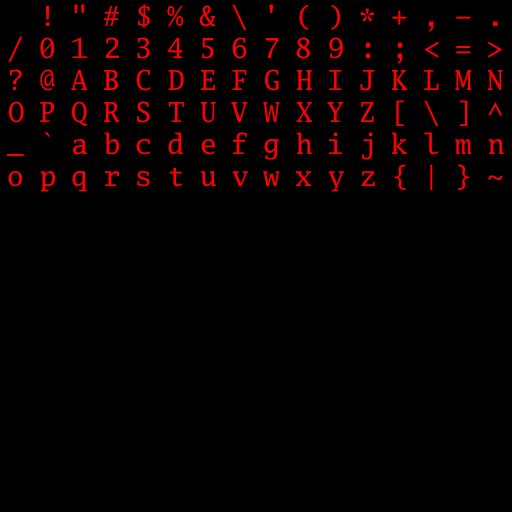
\includegraphics[width=0.5\textwidth]{images/font_texture.png}
	\caption{Przykładowa tekstura dla czcionki Go-Mono \cite{GOMONOFONT} (opracowanie własne)}
	\label{font_texture}
\end{figure}

\subsubsection{Zasób materiału \textit{asset\_material}}
Zasób materiału \textit{asset\_material} reprezentuje parametry używanego podczas renderowania powierzchni
prymitywów przy pomocy następujących parameterów:
\begin{itemize}
	\item \textit{baseColorFactor}: współczynnik koloru podstawowego (vec4);
	\item \textit{metallicFactor}: współczynnik metaliczności zakres, $\left[0,1\right]$;
	\item \textit{roughnessFactor}: współczynnik chropowatości $\left[0,1\right]$;
	\item \textit{metallicRoughnessTexture}: tekstura metaliczności-chropowatości, opcjonalna;
	\item \textit{normalMapTexture}: mapa normalnych, opcjonalna.
\end{itemize}

\subsubsection{Zasób tekstury \textit{asset\_texture}}
Zasób tekstury \textit{asset\_texture} reprezentuje próbkowalny obraz i składa się z zasobu obrazu oraz zasobu próbnika.

\subsubsection{Zasób obrazu \textit{asset\_image}}
Zasób obrazu \textit{asset\_image} zawiera dane obrazu w postaci nieskompresowanej bitmapy.
Bitmapa to prostokątna tablica pikseli opisywana przez następujące parametry:
\begin{itemize}
	\item szerokość i wysokość (uint32\_t);
	\item liczba ścian: domyślnie 1 ściana, 6 ścian dla tekstur sześciennych (uint32\_t);
	\item liczba kanałów: specyfikuje liczbę komponentów i tym samym rozmiar piksela, jeden kanał jest reprezentowany przez jeden bajt (uint32\_t).
\end{itemize}

\subsubsection{Zasób próbnika \textit{asset\_sampler}}
Zasób próbnika \textit{asset\_sampler} reprezentuje parametry używane do stworzenia próbnika obrazu:
\begin{itemize}
	\item \textit{magFilter}: filtr pomniejszający (VkFilter),
	\item \textit{minFilter}: filtr powiększający (VkFilter),
	\item \textit{addressModeU}: tryb adresowania współrzędnych tekstur poza przedziałem $\left[0,1\right]$ dla osi X (VkSamplerAddressMode),
	\item \textit{addressModeV}: tryb adresowania współrzędnych tekstur poza przedziałem $\left[0,1\right]$ dla osi Y (VkSamplerAddressMode),
\end{itemize}

\subsubsection{Potok zasobów asset\_pipeline}
Potok zasobów składa się z dwóch części:
\begin{itemize}
	\item narzędzia wiersza poleceń \textit{asset\_pipeline},
	\item skryptu Python \textit{asset\_pipeline}.
\end{itemize}

Skrypt skanuje podkatalog z zasobami wejściowymi i wywołuje narzędzie z argumentami będącymi ścieżką zasoby wejściowego rodzajem konwertowanego zasobu wyjściowego.
Przykładowo poniższy potok zasobów wywołuje narzędzie 5 razy tworząc pustą konfigurację globalną oraz pustą bazę zasobów wypełnioną zasobem skybox, zasobem czcionki Go-Mono oraz zasobami składającymi się na scenę Sponza opisanej plikiem glTF:
\lstset{language=verbatim}
\begin{lstlisting}[caption={Komeny wywoływane przez przykładowy potok zasobów},captionpos=b]
asset_pipeline empty_config
asset_pipeline empty_assets
asset_pipeline cubemap "skybox1" "/home/user/repo/cmake-build-debug/assets/cubemap/skybox1" png
asset_pipeline font "Go-Mono" "/home/sszczyrb/repo/cmake-build-debug/assets/font/Go-Mono.ttf"
asset_pipeline gltf "sponza" "/home/user/repo/cmake-build-debug/assets/gltf/sponza"
\end{lstlisting}

\subsection{Vulkan}

// TODO Vulkan to moduł zawierajacy 

\subsubsection{Jednostka shader}
Obiekt \textit{shader} reprezentuje pojedynczy shader i jest odpowiedzialny za kompilację ich do formy używalnej przez Vulkan.

Obiekt składa się z następujących elementów:
\begin{itemize}
	\item typ shadera,
	\item kod źródłowy GLSL,
	\item kod bajtowy SPIR-V,
	\item moduł shadera,
	\item obiekt \textit{shader\_reflect}.
\end{itemize}

Typ shadera zależy od tego, dla którego etapu potoku graficznego jest on przeznaczony.
Wspierane są dwa typy: wierzchołków i fragmentów.

Kod źródłowy GLSL must być znany podczas tworzenia - jest on uzyskiwany poprzez użycie obiektu \textit{shader\_generator}.

Kod bajtowy SPIR-V jest uzyskiwany poprzez kompilację kodu źródłowego GLSL biblioteką \textit{shaderc}.
Jej użycie ilustruje poniższy kod:
\lstset{language=C}
\begin{lstlisting}[caption={Kompilacja kodu źródłowego GLSL biblioteką \textit{shaderc}},captionpos=b]
shaderc_compiler_t compiler = shaderc_compiler_initialize();

shaderc_compile_options_t options = shaderc_compile_options_initialize();
shaderc_compile_options_set_target_env(options, shaderc_target_env_vulkan, 0);

const char *glslCode = ...;
size_t glslLen = strlen(glslCode);
shaderc_shader_kind shaderType = ...;
const char *inputFileName = "shader";
const char *entryPointName = "main";
shaderc_compilation_result_t result = shaderc_compile_into_spv(
compiler, glslCode, glslLen,
shaderType, inputFileName, entryPointName, NULL);
shaderc_compile_options_release(options);

if (shaderc_result_get_num_errors(result)) {
	const char *errorMsg = shaderc_result_get_error_message(result);
	panic("compilation error: %s\n", errorMsg);
}

size_t spvSize = shaderc_result_get_length(result);
uint32_t *spvCode = (uint32_t *)malloc(spvSize);
core_memcpy(spvCode, (uint32_t *)shaderc_result_get_bytes(result), spvSize);

shaderc_result_release(result);
shaderc_compiler_release(compiler)
\end{lstlisting}

Moduł shadera jest on uzyskiwany poprzez kompilację kodu bajtowego SPIR-V funkcją vkCreateShaderModule(), który jest też używany do uzyskania obiektu \textit{shader\_reflect}.

\subsubsection{Jednostka shader\_reflect}
Obiekt \textit{shader\_reflect} reprezentuje mechanizm refleksji shadera pozwalający na badanie jego struktury.
Operuje on na kodzie bajtowym SPIR-V i jest on używany podczas testów oraz do logowania informacji debugujących.

\subsection{Scena}

Moduł sceny jest odpowiedzialny za konwersję sceny z wysokopoziomowej formy używanej przez bazę zasobów do niskopoziomowej formy łatwo używalnej przez renderer do wyemitowania polecenia rysowania pośredniego.

Implementacja została zainspirowana techniką modelowania hierarchicznego opracowana w firmie Nvidia \cite{ADVANCEDSCENEGRAPH}.

Scena jest opisywana przy pomocy grafu sceny, którego węzeł zawieraja zasób prymitywu, lokalną trasformację przestrzeni świata oraz węzły potomne.
W tradycyjnym podejściu do modelowania hierarchicznego 
 znajdują się w  przy użyciu grafu sceny
// HIRO

Obiekty biorące udział w procesie konwersji sceny wraz z przepływem danych są przedstawione na poniższym diagramie:
\begin{figure}[H]
	\centering
	\begin{tikzpicture}[node distance=0.5cm]
		\tikzstyle{entity} = [rectangle, minimum width=3cm, minimum height=0.5cm,text centered, draw=black]
		\tikzstyle{flows} = [thick,->,>=stealth]
		
		\node (scene_data) [entity] {scene\_data};
		\node (scene_graph) [entity, below = of scene_data] {scene\_graph};
		\node (scene_tree) [entity, below = of scene_graph] {scene\_tree};
		\node (renderer_cache) [entity, below = of scene_tree] {renderer\_cache};
		
		\node (scene_graph_node) [entity, right = of scene_graph] {scene\_graph\_node};
		\node (scene_graph_node_dots) [right = 1mm of scene_graph_node] {...};
		\node (scene_tree_node) [entity, right = of scene_tree] {scene\_tree\_node};
		\node (scene_tree_node_dots) [right = 1mm of scene_tree_node] {...};
		
		\node (renderer_cache_primitive_element) [entity, below = of renderer_cache] {renderer\_cache\_primitive\_element};
		\node (renderer_cache_primitive_element_dots) [right = 1mm of renderer_cache_primitive_element] {...};
		\node (renderer_cache_camera_element) [entity, below = of renderer_cache_primitive_element] {renderer\_cache\_camera\_element};
		\node (renderer_cache_camera_element_dots) [right = 1mm of renderer_cache_camera_element] {...};
		\node (renderer_cache_direct_light_element) [entity, below = of renderer_cache_camera_element] {renderer\_cache\_direct\_light\_element};
		\node (renderer_cache_direct_light_element_dots) [right = 1mm of renderer_cache_direct_light_element] {...};
		\node (renderer_cache_skybox_element) [entity, below = of renderer_cache_direct_light_element] {renderer\_cache\_skybox\_element};
		\node (renderer_cache_skybox_element_dots) [right = 1mm of renderer_cache_skybox_element] {...};
		\node(renderer_cache_elements)[draw,dotted,fit=(renderer_cache_primitive_element) (renderer_cache_camera_element) (renderer_cache_direct_light_element) (renderer_cache_skybox_element) (renderer_cache_direct_light_element_dots)] {};
		
		\node (vkCmdDrawIndexedIndirect) [entity, right = of renderer_cache_elements] {vkCmdDrawIndexedIndirect()};
		
		\draw [flows] (scene_data) edge[out=-90,in=90] (scene_graph);
		\draw [flows] (scene_graph) edge[out=180,in=180] (renderer_cache);
		\draw [flows] (scene_graph) edge[out=-90,in=90] (scene_tree);
		\draw [flows] (scene_graph) edge[] (scene_graph_node);
		\draw [flows] (scene_graph_node) edge[] (scene_tree_node);
		\draw [flows] (scene_tree) edge[out=-90,in=90] (renderer_cache);
		\draw [flows] (scene_tree) edge[] (scene_tree_node);
		\draw [flows] (renderer_cache) edge[] (renderer_cache_elements);
		\draw [flows] (renderer_cache_elements) edge[] (vkCmdDrawIndexedIndirect);
		// HIRO nodes
		
	\end{tikzpicture}
	\caption{Obiekty biorące udział w procesie konwersji sceny wraz z przepływem danych (opracowanie własne)}
	\label{scene_process}
\end{figure}

\subsubsection{Dane sceny scene\_data}
Obiekt \textit{scene\_data} reprezentuje dane sceny wczytane z bazy zasobów. Jest one używany przez moduł sceny do konstrukcji grafu sceny \textit{scene\_graph}.

Obiekt utrzymuje on dla każdego typu obiektu zasobu osobną listę dwukierunkową zawierającą wszystkie obiekty używane przez scenę oraz ich domyślne warianty. Przykładowo domyślny obraz \textit{asset\_image} to obraz 2D o rozmiarze 1x1 mający 4 8-bitowe komponenty o wartości 255.

Wśród wszystkich obiektów zasobów składających się na dane sceny dodatkowo wyróżnia się:
\begin{itemize}
	\item węzły główne: używane jako punkty początkowe podczas tworzenia grafu sceny,
	\item używany skybox: może być zmieniony w konfiguracji zasobów,
	\item aktywna czcionka: sterowana konfiguracją globalną,
	\item domyślna kamera: używana w przypadku braku węzła z przypisaną kamerą.
\end{itemize}

Metody \textit{serialize()} i \textit{deserialize()} podobnie jak analogiczne metody obiektów zasobów pozwalają na zapis i odczyt danych sceny do bazy zasobów.

Metoda \textit{create\_with\_gltf\_file()} jest wywoływane wyłącznie przez potok zasobów.
Jej wejściem jest nazwa tworzonej sceny i ścieżka do katalogu zawierającego zasób 3D w formacie \textit{glTF} wraz z konfiguracją zasobów.
Oba zasoby wejściowe są parsowane przy użyciu biblioteki \textit{cgltf} i obiektu \textit{config}.
Wynik parsowania jest używany do stworzenia i wypełnienia danych sceny.
Ta metoda wraz z metodą \textit{serialize()} stanowi główną częścią potoku zasobów - obiekt stworzony na podstawie zasobów wejściowych jest serializowany do zasobu wyjściowego (bazy zasobów).

Metoda \textit{create\_with\_asset\_db()} jest wywoływana w czasie wykonywania i wczytuje dane sceny o żądanej nazwie z bazy zasobów.

\subsubsection{Graf sceny scene\_graph}
Obiekt \textit{scene\_graph} reprezentuje
// HIRO

\subsubsection{Drzewo sceny scene\_tree}
Obiekt \textit{scene\_tree} reprezentuje
// HIRO

\subsection{Renderer}

// TODO Renderer to moduł zawierajacy 

// HIRO renderer\_cache

// HIRO Stan renderowania renderer\_state

// HIRO Graf renderowania render\_graph

// HIRO renderer
\chapter{Badania}
\label{chap:research}

// TODO: Prezentacja renderdoc
// TODO: Profiling różne sceny.
// TODO: test: technika filtrowanie anizotropowe, usuń TRANSIENT
// TODO: test: usuń mipmapy, usuń multidraw

\chapter{Podsumowanie}
\label{chap:summary}

Efektem niniejszej pracy jest silnik graficzny pozwalający na renderowanie używając cieniowania odroczonego i innych technik graficznych.
Zrealizowano zamierzone cele dotyczące funkcjonalności silnika oraz zademonstrowano jego działanie poprzez wyrenderowanie przykładowych scen. Przeprowadzono testy wydajnościowe.

// HIRO dobrze byłoby trochę bardziej rozbudować podsumowanie tego, co zostało konkretnie zaimplementowane (2-3 akapity)



Projekt w obecnym kształcie nie został wykorzystany w grze komputerowej i powinien być rozpatrywany w kategoriach prototypu.
Rozwój funkcjonalności silnika nie jest zakończony i w czasie realizacji projektu pojawiło się wiele pomysłów na ulepszenia.

Silnik był napisany i przetestowany wyłącznie na systemie Linux, ale wieloplatformowa natura używanych narzędzi i bibliotek powinna pozwolić na dokonanie kompilacji skrośnej.

Renderer odroczony w obecnym kształcie obsługuje tylko nieprzeźroczyste obiekty. Rysowanie obiektów przeźroczystych mogłoby być rozwiązane dodatkowym przebiegiem renderowania wprzód dla posortowanych obiektów z mieszaniem alfa. Bardziej dokładna, lecz wolniejsza, przeźroczystość dla skomplikowanej geometrii może być osiągnięta używając technik przeźroczystości niezależnej od kolejności (ang. order-independent transparency, OIT).

Wszystkie zasoby są jednokrotnie kopiowane z GPU do CPU przed rozpoczęciem pętli głównej renderowania.
Bardziej efektywnym pamięciowo podejściem byłoby przesyłanie strumieniowe zasobów polegające na ładowaniu ich tylko gdy są rzeczywiście używane do renderowania.

Z przesyłaniem strumieniowym dobrze współpracują techniki usuwania niewidocznych powierzchni.
Najprostszą do implementacji jest odrzucanie na CPU obiektów poza bryłą widzenia pozwalające na niewysyłanie nierenderowanej geometrii do GPU.
Znacznie bardziej skomplikowane, ale zgodne z duchem renderowania bez dowiązań, jest usuwanie niewidocznych powierzchni na GPU. Może być ono zrealizowane w Vulkan używając shaderów obliczeń modyfikujących bufory pośrednie używane przez polecenia rysowania.

Użycie shaderów obliczeń pozwoliłoby też na zastosowanie techniki programowalnego pobierania wierzchołków (ang. programmable vertex pulling) \cite{kosarevsky20213d}, w której etap asemblera wejścia potoku graficznego jest całkowicie pomijany i zastępowany odczytywaniem i dekodowaniem danych geometrii z zasobów shadera.
Podejście to pozwoliłoby na eleminację ujednoliconego bufora geometrii oraz zastąpienie sztywnego definiowania formatów wierzchołków w potoku graficznym elastyczniejszym dekodującym kodem w shaderach. 

Model oświetlenia może być rozszerzony o powierzchnie emitujące światło poprzez dodanie tekstur emisyjnych.
Podobnie tekstury skybox mogą być użyte do mapowania środowiskowego symulującego odbicia światła dla połyskliwych powierzchni.

% Bibliografia, ignorujemy overfull box, bo są długie URL
\hfuzz=50pt
\printbibliography[title=\bibliographyname]
\addcontentsline{toc}{chapter}{\bibliographyname}
\hfuzz=0pt

% Wykaz rysunków
\listoffigures
\addcontentsline{toc}{chapter}{\listfigurename}

% Wykaz tabel
\listoftables
\addcontentsline{toc}{chapter}{\listtablename}

\end{document}
